\documentclass[twoside]{book}

% Packages required by doxygen
\usepackage{fixltx2e}
\usepackage{calc}
\usepackage{doxygen}
\usepackage[export]{adjustbox} % also loads graphicx
\usepackage{graphicx}
\usepackage[utf8]{inputenc}
\usepackage{makeidx}
\usepackage{multicol}
\usepackage{multirow}
\PassOptionsToPackage{warn}{textcomp}
\usepackage{textcomp}
\usepackage[nointegrals]{wasysym}
\usepackage[table]{xcolor}

% Font selection
\usepackage[T1]{fontenc}
\usepackage[scaled=.90]{helvet}
\usepackage{courier}
\usepackage{amssymb}
\usepackage{sectsty}
\renewcommand{\familydefault}{\sfdefault}
\allsectionsfont{%
  \fontseries{bc}\selectfont%
  \color{darkgray}%
}
\renewcommand{\DoxyLabelFont}{%
  \fontseries{bc}\selectfont%
  \color{darkgray}%
}
\newcommand{\+}{\discretionary{\mbox{\scriptsize$\hookleftarrow$}}{}{}}

% Page & text layout
\usepackage{geometry}
\geometry{%
  a4paper,%
  top=2.5cm,%
  bottom=2.5cm,%
  left=2.5cm,%
  right=2.5cm%
}
\tolerance=750
\hfuzz=15pt
\hbadness=750
\setlength{\emergencystretch}{15pt}
\setlength{\parindent}{0cm}
\setlength{\parskip}{3ex plus 2ex minus 2ex}
\makeatletter
\renewcommand{\paragraph}{%
  \@startsection{paragraph}{4}{0ex}{-1.0ex}{1.0ex}{%
    \normalfont\normalsize\bfseries\SS@parafont%
  }%
}
\renewcommand{\subparagraph}{%
  \@startsection{subparagraph}{5}{0ex}{-1.0ex}{1.0ex}{%
    \normalfont\normalsize\bfseries\SS@subparafont%
  }%
}
\makeatother

% Headers & footers
\usepackage{fancyhdr}
\pagestyle{fancyplain}
\fancyhead[LE]{\fancyplain{}{\bfseries\thepage}}
\fancyhead[CE]{\fancyplain{}{}}
\fancyhead[RE]{\fancyplain{}{\bfseries\leftmark}}
\fancyhead[LO]{\fancyplain{}{\bfseries\rightmark}}
\fancyhead[CO]{\fancyplain{}{}}
\fancyhead[RO]{\fancyplain{}{\bfseries\thepage}}
\fancyfoot[LE]{\fancyplain{}{}}
\fancyfoot[CE]{\fancyplain{}{}}
\fancyfoot[RE]{\fancyplain{}{\bfseries\scriptsize Generated by Doxygen }}
\fancyfoot[LO]{\fancyplain{}{\bfseries\scriptsize Generated by Doxygen }}
\fancyfoot[CO]{\fancyplain{}{}}
\fancyfoot[RO]{\fancyplain{}{}}
\renewcommand{\footrulewidth}{0.4pt}
\renewcommand{\chaptermark}[1]{%
  \markboth{#1}{}%
}
\renewcommand{\sectionmark}[1]{%
  \markright{\thesection\ #1}%
}

% Indices & bibliography
\usepackage{natbib}
\usepackage[titles]{tocloft}
\setcounter{tocdepth}{3}
\setcounter{secnumdepth}{5}
\makeindex

% Hyperlinks (required, but should be loaded last)
\usepackage{ifpdf}
\ifpdf
  \usepackage[pdftex,pagebackref=true]{hyperref}
\else
  \usepackage[ps2pdf,pagebackref=true]{hyperref}
\fi
\hypersetup{%
  colorlinks=true,%
  linkcolor=blue,%
  citecolor=blue,%
  unicode%
}

% Custom commands
\newcommand{\clearemptydoublepage}{%
  \newpage{\pagestyle{empty}\cleardoublepage}%
}

\usepackage{caption}
\captionsetup{labelsep=space,justification=centering,font={bf},singlelinecheck=off,skip=4pt,position=top}

%===== C O N T E N T S =====

\begin{document}

% Titlepage & ToC
\hypersetup{pageanchor=false,
             bookmarksnumbered=true,
             pdfencoding=unicode
            }
\pagenumbering{roman}
\begin{titlepage}
\vspace*{7cm}
\begin{center}%
{\Large My Project }\\
\vspace*{1cm}
{\large Generated by Doxygen 1.8.11}\\
\end{center}
\end{titlepage}
\clearemptydoublepage
\tableofcontents
\clearemptydoublepage
\pagenumbering{arabic}
\hypersetup{pageanchor=true}

%--- Begin generated contents ---
\chapter{Hierarchical Index}
\section{Class Hierarchy}
This inheritance list is sorted roughly, but not completely, alphabetically\+:\begin{DoxyCompactList}
\item \contentsline{section}{Amphibia}{\pageref{classAmphibia}}{}
\item \contentsline{section}{Animal}{\pageref{classAnimal}}{}
\begin{DoxyCompactList}
\item \contentsline{section}{Flying\+Animal}{\pageref{classFlyingAnimal}}{}
\begin{DoxyCompactList}
\item \contentsline{section}{Bat}{\pageref{classBat}}{}
\item \contentsline{section}{Cendrawasih}{\pageref{classCendrawasih}}{}
\item \contentsline{section}{Eagle}{\pageref{classEagle}}{}
\item \contentsline{section}{Kolibri}{\pageref{classKolibri}}{}
\end{DoxyCompactList}
\item \contentsline{section}{Land\+Animal}{\pageref{classLandAnimal}}{}
\begin{DoxyCompactList}
\item \contentsline{section}{Cheetah}{\pageref{classCheetah}}{}
\item \contentsline{section}{Chimpanzee}{\pageref{classChimpanzee}}{}
\item \contentsline{section}{Coala}{\pageref{classCoala}}{}
\item \contentsline{section}{Gorilla}{\pageref{classGorilla}}{}
\item \contentsline{section}{Hyena}{\pageref{classHyena}}{}
\item \contentsline{section}{Kangaroo}{\pageref{classKangaroo}}{}
\item \contentsline{section}{Komodo}{\pageref{classKomodo}}{}
\item \contentsline{section}{Lion}{\pageref{classLion}}{}
\item \contentsline{section}{Orangutan}{\pageref{classOrangutan}}{}
\item \contentsline{section}{Ostrich}{\pageref{classOstrich}}{}
\item \contentsline{section}{Panda}{\pageref{classPanda}}{}
\item \contentsline{section}{Peacock}{\pageref{classPeacock}}{}
\item \contentsline{section}{Tiger}{\pageref{classTiger}}{}
\end{DoxyCompactList}
\item \contentsline{section}{Land\+Water\+Animal}{\pageref{classLandWaterAnimal}}{}
\begin{DoxyCompactList}
\item \contentsline{section}{Frog}{\pageref{classFrog}}{}
\end{DoxyCompactList}
\item \contentsline{section}{Water\+Animal}{\pageref{classWaterAnimal}}{}
\begin{DoxyCompactList}
\item \contentsline{section}{Dolphin}{\pageref{classDolphin}}{}
\item \contentsline{section}{Mantaray}{\pageref{classMantaray}}{}
\item \contentsline{section}{Shark}{\pageref{classShark}}{}
\item \contentsline{section}{Whale}{\pageref{classWhale}}{}
\end{DoxyCompactList}
\end{DoxyCompactList}
\item \contentsline{section}{Cage}{\pageref{classCage}}{}
\item \contentsline{section}{cage\+\_\+list}{\pageref{classcage__list}}{}
\item \contentsline{section}{Carnivore}{\pageref{classCarnivore}}{}
\begin{DoxyCompactList}
\item \contentsline{section}{Bat}{\pageref{classBat}}{}
\item \contentsline{section}{Cheetah}{\pageref{classCheetah}}{}
\item \contentsline{section}{Dolphin}{\pageref{classDolphin}}{}
\item \contentsline{section}{Eagle}{\pageref{classEagle}}{}
\item \contentsline{section}{Frog}{\pageref{classFrog}}{}
\item \contentsline{section}{Hyena}{\pageref{classHyena}}{}
\item \contentsline{section}{Komodo}{\pageref{classKomodo}}{}
\item \contentsline{section}{Lion}{\pageref{classLion}}{}
\item \contentsline{section}{Mantaray}{\pageref{classMantaray}}{}
\item \contentsline{section}{Omnivore}{\pageref{classOmnivore}}{}
\begin{DoxyCompactList}
\item \contentsline{section}{Cendrawasih}{\pageref{classCendrawasih}}{}
\item \contentsline{section}{Chimpanzee}{\pageref{classChimpanzee}}{}
\item \contentsline{section}{Gorilla}{\pageref{classGorilla}}{}
\item \contentsline{section}{Kolibri}{\pageref{classKolibri}}{}
\item \contentsline{section}{Orangutan}{\pageref{classOrangutan}}{}
\item \contentsline{section}{Ostrich}{\pageref{classOstrich}}{}
\end{DoxyCompactList}
\item \contentsline{section}{Shark}{\pageref{classShark}}{}
\item \contentsline{section}{Tiger}{\pageref{classTiger}}{}
\item \contentsline{section}{Whale}{\pageref{classWhale}}{}
\end{DoxyCompactList}
\item \contentsline{section}{Driver}{\pageref{classDriver}}{}
\item \contentsline{section}{Herbivore}{\pageref{classHerbivore}}{}
\begin{DoxyCompactList}
\item \contentsline{section}{Coala}{\pageref{classCoala}}{}
\item \contentsline{section}{Kangaroo}{\pageref{classKangaroo}}{}
\item \contentsline{section}{Omnivore}{\pageref{classOmnivore}}{}
\item \contentsline{section}{Panda}{\pageref{classPanda}}{}
\item \contentsline{section}{Peacock}{\pageref{classPeacock}}{}
\end{DoxyCompactList}
\item \contentsline{section}{Point}{\pageref{classPoint}}{}
\item \contentsline{section}{Renderable}{\pageref{classRenderable}}{}
\begin{DoxyCompactList}
\item \contentsline{section}{Cell}{\pageref{classCell}}{}
\begin{DoxyCompactList}
\item \contentsline{section}{Facility}{\pageref{classFacility}}{}
\begin{DoxyCompactList}
\item \contentsline{section}{Park}{\pageref{classPark}}{}
\item \contentsline{section}{Restaurant}{\pageref{classRestaurant}}{}
\item \contentsline{section}{Road}{\pageref{classRoad}}{}
\begin{DoxyCompactList}
\item \contentsline{section}{Entrance}{\pageref{classEntrance}}{}
\item \contentsline{section}{Exit}{\pageref{classExit}}{}
\end{DoxyCompactList}
\end{DoxyCompactList}
\item \contentsline{section}{Habitat}{\pageref{classHabitat}}{}
\begin{DoxyCompactList}
\item \contentsline{section}{Air\+Habitat}{\pageref{classAirHabitat}}{}
\item \contentsline{section}{Land\+Habitat}{\pageref{classLandHabitat}}{}
\item \contentsline{section}{Water\+Habitat}{\pageref{classWaterHabitat}}{}
\end{DoxyCompactList}
\end{DoxyCompactList}
\end{DoxyCompactList}
\item \contentsline{section}{Taxonomy}{\pageref{classTaxonomy}}{}
\begin{DoxyCompactList}
\item \contentsline{section}{Amphibi}{\pageref{classAmphibi}}{}
\begin{DoxyCompactList}
\item \contentsline{section}{Frog}{\pageref{classFrog}}{}
\end{DoxyCompactList}
\item \contentsline{section}{Aves}{\pageref{classAves}}{}
\begin{DoxyCompactList}
\item \contentsline{section}{Cendrawasih}{\pageref{classCendrawasih}}{}
\item \contentsline{section}{Eagle}{\pageref{classEagle}}{}
\item \contentsline{section}{Kolibri}{\pageref{classKolibri}}{}
\item \contentsline{section}{Ostrich}{\pageref{classOstrich}}{}
\item \contentsline{section}{Peacock}{\pageref{classPeacock}}{}
\end{DoxyCompactList}
\item \contentsline{section}{Mammal}{\pageref{classMammal}}{}
\begin{DoxyCompactList}
\item \contentsline{section}{Bat}{\pageref{classBat}}{}
\item \contentsline{section}{Cheetah}{\pageref{classCheetah}}{}
\item \contentsline{section}{Chimpanzee}{\pageref{classChimpanzee}}{}
\item \contentsline{section}{Coala}{\pageref{classCoala}}{}
\item \contentsline{section}{Dolphin}{\pageref{classDolphin}}{}
\item \contentsline{section}{Gorilla}{\pageref{classGorilla}}{}
\item \contentsline{section}{Hyena}{\pageref{classHyena}}{}
\item \contentsline{section}{Kangaroo}{\pageref{classKangaroo}}{}
\item \contentsline{section}{Lion}{\pageref{classLion}}{}
\item \contentsline{section}{Orangutan}{\pageref{classOrangutan}}{}
\item \contentsline{section}{Panda}{\pageref{classPanda}}{}
\item \contentsline{section}{Tiger}{\pageref{classTiger}}{}
\item \contentsline{section}{Whale}{\pageref{classWhale}}{}
\end{DoxyCompactList}
\item \contentsline{section}{Pisces}{\pageref{classPisces}}{}
\begin{DoxyCompactList}
\item \contentsline{section}{Mantaray}{\pageref{classMantaray}}{}
\item \contentsline{section}{Shark}{\pageref{classShark}}{}
\end{DoxyCompactList}
\item \contentsline{section}{Reptile}{\pageref{classReptile}}{}
\begin{DoxyCompactList}
\item \contentsline{section}{Komodo}{\pageref{classKomodo}}{}
\end{DoxyCompactList}
\end{DoxyCompactList}
\item \contentsline{section}{Zoo}{\pageref{classZoo}}{}
\end{DoxyCompactList}

\chapter{Class Index}
\section{Class List}
Here are the classes, structs, unions and interfaces with brief descriptions\+:\begin{DoxyCompactList}
\item\contentsline{section}{\hyperlink{classAirHabitat}{Air\+Habitat} }{\pageref{classAirHabitat}}{}
\item\contentsline{section}{\hyperlink{classAmphibi}{Amphibi} }{\pageref{classAmphibi}}{}
\item\contentsline{section}{\hyperlink{classAmphibia}{Amphibia} }{\pageref{classAmphibia}}{}
\item\contentsline{section}{\hyperlink{classAnimal}{Animal} }{\pageref{classAnimal}}{}
\item\contentsline{section}{\hyperlink{classAves}{Aves} }{\pageref{classAves}}{}
\item\contentsline{section}{\hyperlink{classBat}{Bat} }{\pageref{classBat}}{}
\item\contentsline{section}{\hyperlink{classCage}{Cage} }{\pageref{classCage}}{}
\item\contentsline{section}{\hyperlink{classcage__list}{cage\+\_\+list} }{\pageref{classcage__list}}{}
\item\contentsline{section}{\hyperlink{classCarnivore}{Carnivore} }{\pageref{classCarnivore}}{}
\item\contentsline{section}{\hyperlink{classCell}{Cell} }{\pageref{classCell}}{}
\item\contentsline{section}{\hyperlink{classCendrawasih}{Cendrawasih} }{\pageref{classCendrawasih}}{}
\item\contentsline{section}{\hyperlink{classCheetah}{Cheetah} }{\pageref{classCheetah}}{}
\item\contentsline{section}{\hyperlink{classChimpanzee}{Chimpanzee} }{\pageref{classChimpanzee}}{}
\item\contentsline{section}{\hyperlink{classCoala}{Coala} }{\pageref{classCoala}}{}
\item\contentsline{section}{\hyperlink{classDolphin}{Dolphin} }{\pageref{classDolphin}}{}
\item\contentsline{section}{\hyperlink{classDriver}{Driver} }{\pageref{classDriver}}{}
\item\contentsline{section}{\hyperlink{classEagle}{Eagle} }{\pageref{classEagle}}{}
\item\contentsline{section}{\hyperlink{classEntrance}{Entrance} }{\pageref{classEntrance}}{}
\item\contentsline{section}{\hyperlink{classExit}{Exit} }{\pageref{classExit}}{}
\item\contentsline{section}{\hyperlink{classFacility}{Facility} }{\pageref{classFacility}}{}
\item\contentsline{section}{\hyperlink{classFlyingAnimal}{Flying\+Animal} }{\pageref{classFlyingAnimal}}{}
\item\contentsline{section}{\hyperlink{classFrog}{Frog} }{\pageref{classFrog}}{}
\item\contentsline{section}{\hyperlink{classGorilla}{Gorilla} }{\pageref{classGorilla}}{}
\item\contentsline{section}{\hyperlink{classHabitat}{Habitat} }{\pageref{classHabitat}}{}
\item\contentsline{section}{\hyperlink{classHerbivore}{Herbivore} }{\pageref{classHerbivore}}{}
\item\contentsline{section}{\hyperlink{classHyena}{Hyena} }{\pageref{classHyena}}{}
\item\contentsline{section}{\hyperlink{classKangaroo}{Kangaroo} }{\pageref{classKangaroo}}{}
\item\contentsline{section}{\hyperlink{classKolibri}{Kolibri} }{\pageref{classKolibri}}{}
\item\contentsline{section}{\hyperlink{classKomodo}{Komodo} }{\pageref{classKomodo}}{}
\item\contentsline{section}{\hyperlink{classLandAnimal}{Land\+Animal} }{\pageref{classLandAnimal}}{}
\item\contentsline{section}{\hyperlink{classLandHabitat}{Land\+Habitat} }{\pageref{classLandHabitat}}{}
\item\contentsline{section}{\hyperlink{classLandWaterAnimal}{Land\+Water\+Animal} }{\pageref{classLandWaterAnimal}}{}
\item\contentsline{section}{\hyperlink{classLion}{Lion} }{\pageref{classLion}}{}
\item\contentsline{section}{\hyperlink{classMammal}{Mammal} }{\pageref{classMammal}}{}
\item\contentsline{section}{\hyperlink{classMantaray}{Mantaray} }{\pageref{classMantaray}}{}
\item\contentsline{section}{\hyperlink{classOmnivore}{Omnivore} }{\pageref{classOmnivore}}{}
\item\contentsline{section}{\hyperlink{classOrangutan}{Orangutan} }{\pageref{classOrangutan}}{}
\item\contentsline{section}{\hyperlink{classOstrich}{Ostrich} }{\pageref{classOstrich}}{}
\item\contentsline{section}{\hyperlink{classPanda}{Panda} }{\pageref{classPanda}}{}
\item\contentsline{section}{\hyperlink{classPark}{Park} }{\pageref{classPark}}{}
\item\contentsline{section}{\hyperlink{classPeacock}{Peacock} }{\pageref{classPeacock}}{}
\item\contentsline{section}{\hyperlink{classPisces}{Pisces} }{\pageref{classPisces}}{}
\item\contentsline{section}{\hyperlink{classPoint}{Point} }{\pageref{classPoint}}{}
\item\contentsline{section}{\hyperlink{classRenderable}{Renderable} }{\pageref{classRenderable}}{}
\item\contentsline{section}{\hyperlink{classReptile}{Reptile} }{\pageref{classReptile}}{}
\item\contentsline{section}{\hyperlink{classRestaurant}{Restaurant} }{\pageref{classRestaurant}}{}
\item\contentsline{section}{\hyperlink{classRoad}{Road} }{\pageref{classRoad}}{}
\item\contentsline{section}{\hyperlink{classShark}{Shark} }{\pageref{classShark}}{}
\item\contentsline{section}{\hyperlink{classTaxonomy}{Taxonomy} }{\pageref{classTaxonomy}}{}
\item\contentsline{section}{\hyperlink{classTiger}{Tiger} }{\pageref{classTiger}}{}
\item\contentsline{section}{\hyperlink{classWaterAnimal}{Water\+Animal} }{\pageref{classWaterAnimal}}{}
\item\contentsline{section}{\hyperlink{classWaterHabitat}{Water\+Habitat} }{\pageref{classWaterHabitat}}{}
\item\contentsline{section}{\hyperlink{classWhale}{Whale} }{\pageref{classWhale}}{}
\item\contentsline{section}{\hyperlink{classZoo}{Zoo} }{\pageref{classZoo}}{}
\end{DoxyCompactList}

\chapter{Class Documentation}
\hypertarget{classAirHabitat}{}\section{Air\+Habitat Class Reference}
\label{classAirHabitat}\index{Air\+Habitat@{Air\+Habitat}}


{\ttfamily \#include $<$Habitat.\+h$>$}



Inheritance diagram for Air\+Habitat\+:

\hypertarget{classAmphibi}{}\section{Amphibi Class Reference}
\label{classAmphibi}\index{Amphibi@{Amphibi}}


Inheritance diagram for Amphibi\+:
\nopagebreak
\begin{figure}[H]
\begin{center}
\leavevmode
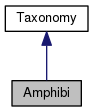
\includegraphics[width=178pt]{classAmphibi__inherit__graph}
\end{center}
\end{figure}


Collaboration diagram for Amphibi\+:
\nopagebreak
\begin{figure}[H]
\begin{center}
\leavevmode
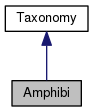
\includegraphics[width=178pt]{classAmphibi__coll__graph}
\end{center}
\end{figure}
\subsection*{Public Member Functions}
\begin{DoxyCompactItemize}
\item 
void \hyperlink{classAmphibi_aee82336be6761e469bbab4388c806bc3}{show\+Tax\+Name} ()\hypertarget{classAmphibi_aee82336be6761e469bbab4388c806bc3}{}\label{classAmphibi_aee82336be6761e469bbab4388c806bc3}

\begin{DoxyCompactList}\small\item\em method show\+Name. Menampilkan nama taksonomi. \end{DoxyCompactList}\end{DoxyCompactItemize}


The documentation for this class was generated from the following files\+:\begin{DoxyCompactItemize}
\item 
Taxonomy.\+h\item 
Taxonomy.\+cpp\end{DoxyCompactItemize}

\hypertarget{classAmphibia}{}\section{Amphibia Class Reference}
\label{classAmphibia}\index{Amphibia@{Amphibia}}


{\ttfamily \#include $<$amphibi.\+h$>$}



Collaboration diagram for Amphibia\+:
% FIG 0


\subsection{Detailed Description}
Base class 

The documentation for this class was generated from the following file\+:\begin{DoxyCompactItemize}
\item 
amphibi/amphibi.\+h\end{DoxyCompactItemize}

\hypertarget{classAnimal}{}\section{Animal Class Reference}
\label{classAnimal}\index{Animal@{Animal}}


{\ttfamily \#include $<$Animal.\+h$>$}



Inheritance diagram for Animal\+:
\nopagebreak
\begin{figure}[H]
\begin{center}
\leavevmode
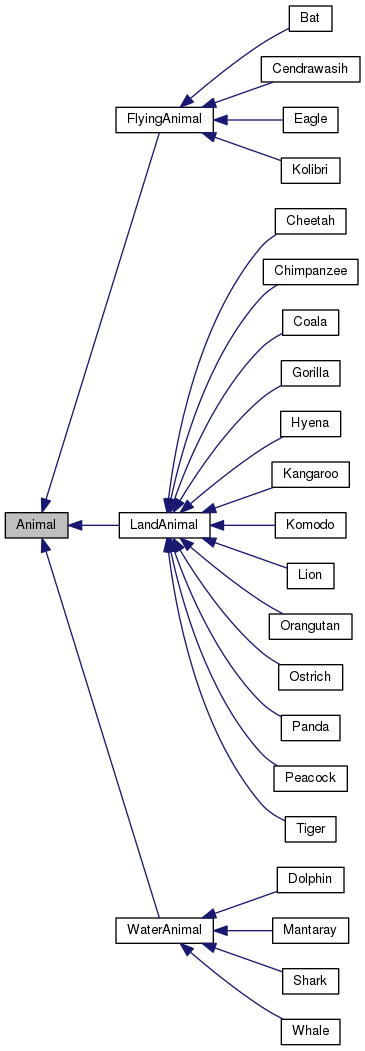
\includegraphics[height=550pt]{classAnimal__inherit__graph}
\end{center}
\end{figure}


Collaboration diagram for Animal\+:
\nopagebreak
\begin{figure}[H]
\begin{center}
\leavevmode
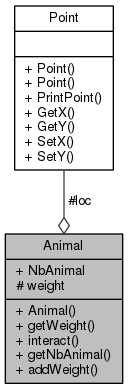
\includegraphics[width=127pt]{classAnimal__coll__graph}
\end{center}
\end{figure}
\subsection*{Public Member Functions}
\begin{DoxyCompactItemize}
\item 
\hyperlink{classAnimal_a38f8dc7a0844d03658f0cd5de482a5db}{Animal} (int x, int y, int w)\hypertarget{classAnimal_a38f8dc7a0844d03658f0cd5de482a5db}{}\label{classAnimal_a38f8dc7a0844d03658f0cd5de482a5db}

\begin{DoxyCompactList}\small\item\em Constructor. Konstruktor kelas animal. \end{DoxyCompactList}\item 
virtual void \hyperlink{classAnimal_af47626b050b665e9a19525227d2b840f}{interact} ()=0\hypertarget{classAnimal_af47626b050b665e9a19525227d2b840f}{}\label{classAnimal_af47626b050b665e9a19525227d2b840f}

\begin{DoxyCompactList}\small\item\em Method interaksi animal. Setiap animal akan berinteraksi dengan cara yang berbeda-\/beda. \end{DoxyCompactList}\item 
int {\bfseries get\+Nb\+Animal} ()\hypertarget{classAnimal_a654785ec6e23f33780711446eff77c81}{}\label{classAnimal_a654785ec6e23f33780711446eff77c81}

\end{DoxyCompactItemize}
\subsection*{Static Public Attributes}
\begin{DoxyCompactItemize}
\item 
static int {\bfseries Nb\+Animal} = 0\hypertarget{classAnimal_a828b89505d3cf5fee0e3042332a81e6e}{}\label{classAnimal_a828b89505d3cf5fee0e3042332a81e6e}

\end{DoxyCompactItemize}
\subsection*{Protected Attributes}
\begin{DoxyCompactItemize}
\item 
\hyperlink{classPoint}{Point} \hyperlink{classAnimal_a7f26dd7aa22ec6c003e0d564fb27baa3}{loc}
\end{DoxyCompactItemize}


\subsection{Detailed Description}
A\+BC animal 

\subsection{Member Data Documentation}
\index{Animal@{Animal}!loc@{loc}}
\index{loc@{loc}!Animal@{Animal}}
\subsubsection[{\texorpdfstring{loc}{loc}}]{\setlength{\rightskip}{0pt plus 5cm}{\bf Point} Animal\+::loc\hspace{0.3cm}{\ttfamily [protected]}}\hypertarget{classAnimal_a7f26dd7aa22ec6c003e0d564fb27baa3}{}\label{classAnimal_a7f26dd7aa22ec6c003e0d564fb27baa3}
Jumlah animal dalam zoo 

The documentation for this class was generated from the following files\+:\begin{DoxyCompactItemize}
\item 
Animal.\+h\item 
Animal.\+cpp\end{DoxyCompactItemize}

\hypertarget{classAves}{}\section{Aves Class Reference}
\label{classAves}\index{Aves@{Aves}}


{\ttfamily \#include $<$aves.\+h$>$}



Inheritance diagram for Aves\+:
% FIG 0


Collaboration diagram for Aves\+:
% FIG 1
\subsection*{Public Member Functions}
\begin{DoxyCompactItemize}
\item 
void \hyperlink{classAves_a6a1aa2435bf6b8f1ef7957c70a86e22e}{Show\+Tax\+Name} ()\hypertarget{classAves_a6a1aa2435bf6b8f1ef7957c70a86e22e}{}\label{classAves_a6a1aa2435bf6b8f1ef7957c70a86e22e}

\begin{DoxyCompactList}\small\item\em method Show\+Name. Menampilkan nama taksonomi. \end{DoxyCompactList}\end{DoxyCompactItemize}


\subsection{Detailed Description}
Base class 

The documentation for this class was generated from the following files\+:\begin{DoxyCompactItemize}
\item 
aves/aves.\+h\item 
aves/aves.\+cpp\end{DoxyCompactItemize}

\hypertarget{classBat}{}\section{Bat Class Reference}
\label{classBat}\index{Bat@{Bat}}


{\ttfamily \#include $<$Flying\+Animal.\+h$>$}



Inheritance diagram for Bat\+:
\nopagebreak
\begin{figure}[H]
\begin{center}
\leavevmode
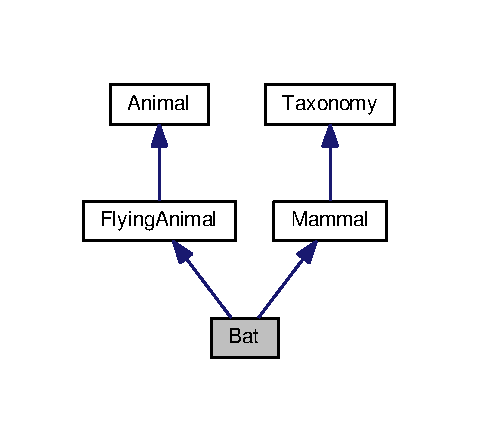
\includegraphics[width=284pt]{classBat__inherit__graph}
\end{center}
\end{figure}


Collaboration diagram for Bat\+:
\nopagebreak
\begin{figure}[H]
\begin{center}
\leavevmode
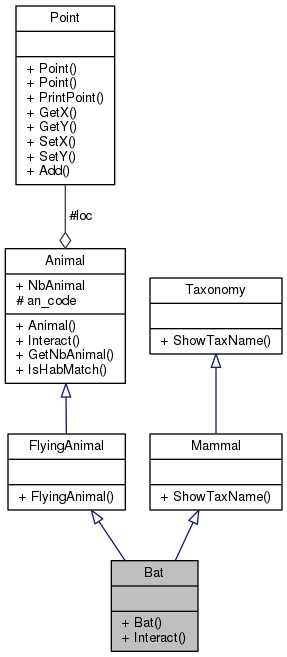
\includegraphics[width=284pt]{classBat__coll__graph}
\end{center}
\end{figure}
\subsection*{Public Member Functions}
\begin{DoxyCompactItemize}
\item 
\hyperlink{classBat_a5d54305430e0d7a6e104a3fd5a944945}{Bat} (int x, int y)
\begin{DoxyCompactList}\small\item\em Constructor. \end{DoxyCompactList}\item 
void \hyperlink{classBat_adf63bb33699532d83e680252c4b7021c}{interact} ()\hypertarget{classBat_adf63bb33699532d83e680252c4b7021c}{}\label{classBat_adf63bb33699532d83e680252c4b7021c}

\begin{DoxyCompactList}\small\item\em Method interaksi bat. \end{DoxyCompactList}\end{DoxyCompactItemize}
\subsection*{Additional Inherited Members}


\subsection{Detailed Description}
Real class bat 

\subsection{Constructor \& Destructor Documentation}
\index{Bat@{Bat}!Bat@{Bat}}
\index{Bat@{Bat}!Bat@{Bat}}
\subsubsection[{\texorpdfstring{Bat(int x, int y)}{Bat(int x, int y)}}]{\setlength{\rightskip}{0pt plus 5cm}Bat\+::\+Bat (
\begin{DoxyParamCaption}
\item[{int}]{x, }
\item[{int}]{y}
\end{DoxyParamCaption}
)}\hypertarget{classBat_a5d54305430e0d7a6e104a3fd5a944945}{}\label{classBat_a5d54305430e0d7a6e104a3fd5a944945}


Constructor. 


\begin{DoxyParams}{Parameters}
{\em x} & absis lokasi \\
\hline
{\em y} & ordinat lokasi Konstruktor kelas bat \\
\hline
\end{DoxyParams}


The documentation for this class was generated from the following files\+:\begin{DoxyCompactItemize}
\item 
Flying\+Animal.\+h\item 
Flying\+Animal.\+cpp\end{DoxyCompactItemize}

\hypertarget{classCage}{}\section{Cage Class Reference}
\label{classCage}\index{Cage@{Cage}}


{\ttfamily \#include $<$Cage.\+h$>$}



Collaboration diagram for Cage\+:
\nopagebreak
\begin{figure}[H]
\begin{center}
\leavevmode
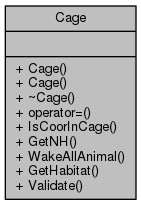
\includegraphics[width=176pt]{classCage__coll__graph}
\end{center}
\end{figure}
\subsection*{Public Member Functions}
\begin{DoxyCompactItemize}
\item 
\hyperlink{classCage_a87cfc71acde51257611ce288e6337363}{Cage} (\hyperlink{classHabitat}{Habitat} $\ast$$\ast$hl, int n)
\begin{DoxyCompactList}\small\item\em Constructor berparameter. Membuat objek cage dengan daftar animal dan habitat yang terdefinisi. \end{DoxyCompactList}\item 
\hyperlink{classCage_ae85bb53517616422bf7f36282de01519}{Cage} (const \hyperlink{classCage}{Cage} \&c)\hypertarget{classCage_ae85bb53517616422bf7f36282de01519}{}\label{classCage_ae85bb53517616422bf7f36282de01519}

\begin{DoxyCompactList}\small\item\em Copy\+Constructor. \end{DoxyCompactList}\item 
\hyperlink{classCage_a657259499dfc23c63fc65aeaf8abbb17}{$\sim$\+Cage} ()\hypertarget{classCage_a657259499dfc23c63fc65aeaf8abbb17}{}\label{classCage_a657259499dfc23c63fc65aeaf8abbb17}

\begin{DoxyCompactList}\small\item\em Destructor. \end{DoxyCompactList}\item 
\hyperlink{classCage}{Cage} \& \hyperlink{classCage_a020eefd2b5d15915cf65693413be64db}{operator=} (const \hyperlink{classCage}{Cage} \&c)\hypertarget{classCage_a020eefd2b5d15915cf65693413be64db}{}\label{classCage_a020eefd2b5d15915cf65693413be64db}

\begin{DoxyCompactList}\small\item\em Operator=. \end{DoxyCompactList}\item 
void {\bfseries wake\+All\+Animal} ()\hypertarget{classCage_a1f5ebc229af63a1b24f596cf919e3f56}{}\label{classCage_a1f5ebc229af63a1b24f596cf919e3f56}

\end{DoxyCompactItemize}


\subsection{Detailed Description}
Kelas yang merepresentasikan kandang dalam zoo. 

\subsection{Constructor \& Destructor Documentation}
\index{Cage@{Cage}!Cage@{Cage}}
\index{Cage@{Cage}!Cage@{Cage}}
\subsubsection[{\texorpdfstring{Cage(\+Habitat $\ast$$\ast$hl, int n)}{Cage(Habitat **hl, int n)}}]{\setlength{\rightskip}{0pt plus 5cm}Cage\+::\+Cage (
\begin{DoxyParamCaption}
\item[{{\bf Habitat} $\ast$$\ast$}]{hl, }
\item[{int}]{n}
\end{DoxyParamCaption}
)}\hypertarget{classCage_a87cfc71acde51257611ce288e6337363}{}\label{classCage_a87cfc71acde51257611ce288e6337363}


Constructor berparameter. Membuat objek cage dengan daftar animal dan habitat yang terdefinisi. 


\begin{DoxyParams}{Parameters}
{\em AL} & List of animal yang berada dalam cage \\
\hline
{\em HL} & List of habitat yang dilingkupi oleh cage na = A\+L.\+size(), nh = H\+L.\+size() \\
\hline
\end{DoxyParams}


The documentation for this class was generated from the following files\+:\begin{DoxyCompactItemize}
\item 
Cage.\+h\item 
Cage.\+cpp\end{DoxyCompactItemize}

\hypertarget{classcage__list}{}\section{cage\+\_\+list Class Reference}
\label{classcage__list}\index{cage\+\_\+list@{cage\+\_\+list}}


Collaboration diagram for cage\+\_\+list\+:
% FIG 0
\subsection*{Public Member Functions}
\begin{DoxyCompactItemize}
\item 
void {\bfseries Add\+Cage} (\hyperlink{classCage}{Cage} c)\hypertarget{classcage__list_a6a936c28a8631dbe1075493ad52e0a31}{}\label{classcage__list_a6a936c28a8631dbe1075493ad52e0a31}

\item 
\hyperlink{classCage}{Cage} \& {\bfseries Get\+Cage} (int i)\hypertarget{classcage__list_a01ec3086049a333334a49b385587c50a}{}\label{classcage__list_a01ec3086049a333334a49b385587c50a}

\item 
int {\bfseries Get\+Size} ()\hypertarget{classcage__list_ad081b5200e87142d4805004fcdaf5056}{}\label{classcage__list_ad081b5200e87142d4805004fcdaf5056}

\item 
int {\bfseries Search\+By\+Coor} (int x, int y)\hypertarget{classcage__list_aa44cc46a9811038a3a48cb7968d4dd30}{}\label{classcage__list_aa44cc46a9811038a3a48cb7968d4dd30}

\item 
bool {\bfseries Is\+Overlap} (const \hyperlink{classCage}{Cage} \&c)\hypertarget{classcage__list_a881e87209a22c09d3716db482b9e469f}{}\label{classcage__list_a881e87209a22c09d3716db482b9e469f}

\end{DoxyCompactItemize}


The documentation for this class was generated from the following files\+:\begin{DoxyCompactItemize}
\item 
cage\+\_\+list/cage\+\_\+list.\+h\item 
cage\+\_\+list/cage\+\_\+list.\+cpp\end{DoxyCompactItemize}

\hypertarget{classCarnivore}{}\section{Carnivore Class Reference}
\label{classCarnivore}\index{Carnivore@{Carnivore}}


{\ttfamily \#include $<$carnivore.\+h$>$}



Inheritance diagram for Carnivore\+:
% FIG 0


Collaboration diagram for Carnivore\+:
% FIG 1
\subsection*{Public Member Functions}
\begin{DoxyCompactItemize}
\item 
\hyperlink{classCarnivore_a2346389567a28181cd49894a56834979}{Carnivore} (int weight)
\begin{DoxyCompactList}\small\item\em Constructor. \end{DoxyCompactList}\item 
float \hyperlink{classCarnivore_a1032e38dee235a21c3a6b5d77e9a7906}{Get\+Food} () const \hypertarget{classCarnivore_a1032e38dee235a21c3a6b5d77e9a7906}{}\label{classCarnivore_a1032e38dee235a21c3a6b5d77e9a7906}

\begin{DoxyCompactList}\small\item\em Method Get\+Food mengembalikan makanan karnivora. \end{DoxyCompactList}\end{DoxyCompactItemize}
\subsection*{Static Public Attributes}
\begin{DoxyCompactItemize}
\item 
static int \hyperlink{classCarnivore_ad134bd8ca67aed9b5fd59be18d8ae8b7}{n\+\_\+carnivore} = 0
\item 
static float \hyperlink{classCarnivore_ab449b336745a74e84784bfc13489ec15}{total\+\_\+cfood} = 0
\end{DoxyCompactItemize}
\subsection*{Protected Attributes}
\begin{DoxyCompactItemize}
\item 
float \hyperlink{classCarnivore_af1b6929b2e0d7204ad0c0a865fe6e96b}{cfood}
\end{DoxyCompactItemize}


\subsection{Detailed Description}
Base class carnivore 

\subsection{Constructor \& Destructor Documentation}
\index{Carnivore@{Carnivore}!Carnivore@{Carnivore}}
\index{Carnivore@{Carnivore}!Carnivore@{Carnivore}}
\subsubsection[{\texorpdfstring{Carnivore(int weight)}{Carnivore(int weight)}}]{\setlength{\rightskip}{0pt plus 5cm}Carnivore\+::\+Carnivore (
\begin{DoxyParamCaption}
\item[{int}]{weight}
\end{DoxyParamCaption}
)}\hypertarget{classCarnivore_a2346389567a28181cd49894a56834979}{}\label{classCarnivore_a2346389567a28181cd49894a56834979}


Constructor. 


\begin{DoxyParams}{Parameters}
{\em weight} & Konstruktor carnivore dengan parameter berat badan \\
\hline
\end{DoxyParams}


\subsection{Member Data Documentation}
\index{Carnivore@{Carnivore}!cfood@{cfood}}
\index{cfood@{cfood}!Carnivore@{Carnivore}}
\subsubsection[{\texorpdfstring{cfood}{cfood}}]{\setlength{\rightskip}{0pt plus 5cm}float Carnivore\+::cfood\hspace{0.3cm}{\ttfamily [protected]}}\hypertarget{classCarnivore_af1b6929b2e0d7204ad0c0a865fe6e96b}{}\label{classCarnivore_af1b6929b2e0d7204ad0c0a865fe6e96b}
Makanan karnivora \index{Carnivore@{Carnivore}!n\+\_\+carnivore@{n\+\_\+carnivore}}
\index{n\+\_\+carnivore@{n\+\_\+carnivore}!Carnivore@{Carnivore}}
\subsubsection[{\texorpdfstring{n\+\_\+carnivore}{n_carnivore}}]{\setlength{\rightskip}{0pt plus 5cm}int Carnivore\+::n\+\_\+carnivore = 0\hspace{0.3cm}{\ttfamily [static]}}\hypertarget{classCarnivore_ad134bd8ca67aed9b5fd59be18d8ae8b7}{}\label{classCarnivore_ad134bd8ca67aed9b5fd59be18d8ae8b7}
Jumlah hewan karnivora \index{Carnivore@{Carnivore}!total\+\_\+cfood@{total\+\_\+cfood}}
\index{total\+\_\+cfood@{total\+\_\+cfood}!Carnivore@{Carnivore}}
\subsubsection[{\texorpdfstring{total\+\_\+cfood}{total_cfood}}]{\setlength{\rightskip}{0pt plus 5cm}float Carnivore\+::total\+\_\+cfood = 0\hspace{0.3cm}{\ttfamily [static]}}\hypertarget{classCarnivore_ab449b336745a74e84784bfc13489ec15}{}\label{classCarnivore_ab449b336745a74e84784bfc13489ec15}
Jumlah total makanan karnivora 

The documentation for this class was generated from the following files\+:\begin{DoxyCompactItemize}
\item 
carnivore/carnivore.\+h\item 
carnivore/carnivore.\+cpp\end{DoxyCompactItemize}

\hypertarget{classCell}{}\section{Cell Class Reference}
\label{classCell}\index{Cell@{Cell}}


{\ttfamily \#include $<$Cell.\+h$>$}



Inheritance diagram for Cell\+:
\nopagebreak
\begin{figure}[H]
\begin{center}
\leavevmode
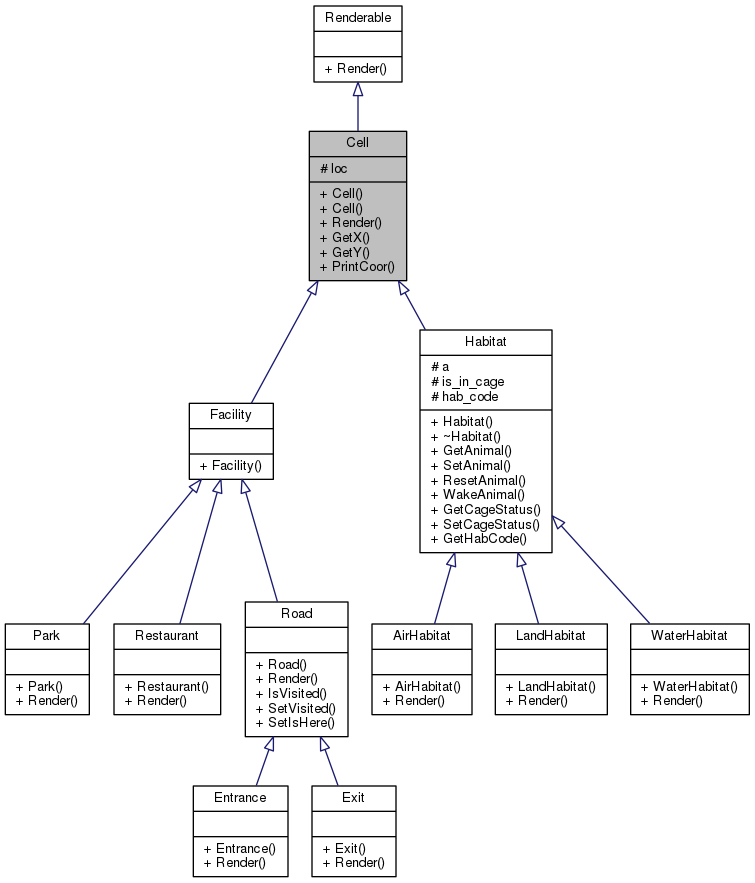
\includegraphics[width=350pt]{classCell__inherit__graph}
\end{center}
\end{figure}


Collaboration diagram for Cell\+:
\nopagebreak
\begin{figure}[H]
\begin{center}
\leavevmode
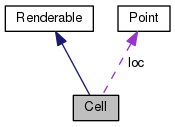
\includegraphics[width=238pt]{classCell__coll__graph}
\end{center}
\end{figure}
\subsection*{Public Member Functions}
\begin{DoxyCompactItemize}
\item 
\hyperlink{classCell_a394510643e8664cf12b5efaf5cb99f71}{Cell} ()\hypertarget{classCell_a394510643e8664cf12b5efaf5cb99f71}{}\label{classCell_a394510643e8664cf12b5efaf5cb99f71}

\begin{DoxyCompactList}\small\item\em Constructor. Membuat objek bertipe \hyperlink{classCell}{Cell} dengan menginisialisasi koordinatnya menjadi (0,0) \end{DoxyCompactList}\item 
\hyperlink{classCell_aa39ad04eeebb7bf00d592ad36640337e}{Cell} (int x, int y)
\begin{DoxyCompactList}\small\item\em Constructor. Membuat objek bertipe \hyperlink{classCell}{Cell} dengan menginisialisasi koordinatnya menjadi (x,y) \end{DoxyCompactList}\item 
virtual void {\bfseries render} ()\hypertarget{classCell_a3c55fdf9c9a14cd07e210a2a3fb102ac}{}\label{classCell_a3c55fdf9c9a14cd07e210a2a3fb102ac}

\item 
void {\bfseries print\+Coor} ()\hypertarget{classCell_a184dee133b16168d2ea242d20db79576}{}\label{classCell_a184dee133b16168d2ea242d20db79576}

\end{DoxyCompactItemize}
\subsection*{Protected Attributes}
\begin{DoxyCompactItemize}
\item 
\hyperlink{classPoint}{Point} {\bfseries loc}\hypertarget{classCell_a6955983511c6709d8f5b82b4ba6edb77}{}\label{classCell_a6955983511c6709d8f5b82b4ba6edb77}

\end{DoxyCompactItemize}


\subsection{Detailed Description}
Kelas yang merepresentasikan sel dalam matriks \hyperlink{classZoo}{Zoo}. 

\subsection{Constructor \& Destructor Documentation}
\index{Cell@{Cell}!Cell@{Cell}}
\index{Cell@{Cell}!Cell@{Cell}}
\subsubsection[{\texorpdfstring{Cell(int x, int y)}{Cell(int x, int y)}}]{\setlength{\rightskip}{0pt plus 5cm}Cell\+::\+Cell (
\begin{DoxyParamCaption}
\item[{int}]{x, }
\item[{int}]{y}
\end{DoxyParamCaption}
)}\hypertarget{classCell_aa39ad04eeebb7bf00d592ad36640337e}{}\label{classCell_aa39ad04eeebb7bf00d592ad36640337e}


Constructor. Membuat objek bertipe \hyperlink{classCell}{Cell} dengan menginisialisasi koordinatnya menjadi (x,y) 


\begin{DoxyParams}{Parameters}
{\em x} & absis dari koordinat \hyperlink{classCell}{Cell} \\
\hline
{\em y} & ordinat dari koordinat \hyperlink{classCell}{Cell} \\
\hline
\end{DoxyParams}


The documentation for this class was generated from the following files\+:\begin{DoxyCompactItemize}
\item 
Cell.\+h\item 
Cell.\+cpp\end{DoxyCompactItemize}

\hypertarget{classCendrawasih}{}\section{Cendrawasih Class Reference}
\label{classCendrawasih}\index{Cendrawasih@{Cendrawasih}}


{\ttfamily \#include $<$Flying\+Animal.\+h$>$}



Inheritance diagram for Cendrawasih\+:
% FIG 0


Collaboration diagram for Cendrawasih\+:
% FIG 1
\subsection*{Public Member Functions}
\begin{DoxyCompactItemize}
\item 
\hyperlink{classCendrawasih_a4ccdd43fd72f96b5f7ef32a8dfc7f299}{Cendrawasih} (int x, int y)
\begin{DoxyCompactList}\small\item\em Constructor. \end{DoxyCompactList}\item 
void \hyperlink{classCendrawasih_ab24c4c34838000da51a810dec7d29669}{interact} ()\hypertarget{classCendrawasih_ab24c4c34838000da51a810dec7d29669}{}\label{classCendrawasih_ab24c4c34838000da51a810dec7d29669}

\begin{DoxyCompactList}\small\item\em Method interaksi cendrawasih. \end{DoxyCompactList}\end{DoxyCompactItemize}
\subsection*{Additional Inherited Members}


\subsection{Detailed Description}
Real class cendrawasih 

\subsection{Constructor \& Destructor Documentation}
\index{Cendrawasih@{Cendrawasih}!Cendrawasih@{Cendrawasih}}
\index{Cendrawasih@{Cendrawasih}!Cendrawasih@{Cendrawasih}}
\subsubsection[{\texorpdfstring{Cendrawasih(int x, int y)}{Cendrawasih(int x, int y)}}]{\setlength{\rightskip}{0pt plus 5cm}Cendrawasih\+::\+Cendrawasih (
\begin{DoxyParamCaption}
\item[{int}]{x, }
\item[{int}]{y}
\end{DoxyParamCaption}
)}\hypertarget{classCendrawasih_a4ccdd43fd72f96b5f7ef32a8dfc7f299}{}\label{classCendrawasih_a4ccdd43fd72f96b5f7ef32a8dfc7f299}


Constructor. 


\begin{DoxyParams}{Parameters}
{\em x} & absis lokasi \\
\hline
{\em y} & ordinat lokasi Konstruktor kelas cendrawasih \\
\hline
\end{DoxyParams}


The documentation for this class was generated from the following files\+:\begin{DoxyCompactItemize}
\item 
Flying\+Animal.\+h\item 
Flying\+Animal.\+cpp\end{DoxyCompactItemize}

\hypertarget{classCheetah}{}\section{Cheetah Class Reference}
\label{classCheetah}\index{Cheetah@{Cheetah}}


{\ttfamily \#include $<$Land\+Animal.\+h$>$}



Inheritance diagram for Cheetah\+:
\nopagebreak
\begin{figure}[H]
\begin{center}
\leavevmode
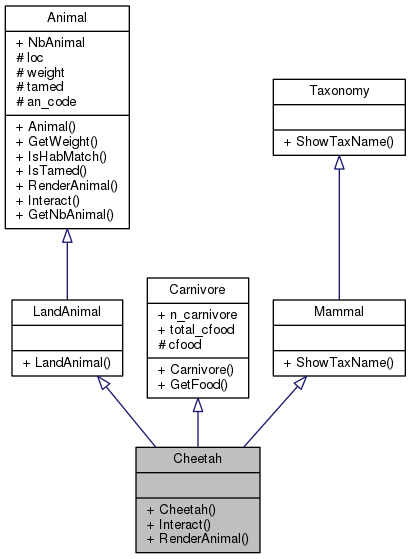
\includegraphics[width=224pt]{classCheetah__inherit__graph}
\end{center}
\end{figure}


Collaboration diagram for Cheetah\+:
\nopagebreak
\begin{figure}[H]
\begin{center}
\leavevmode
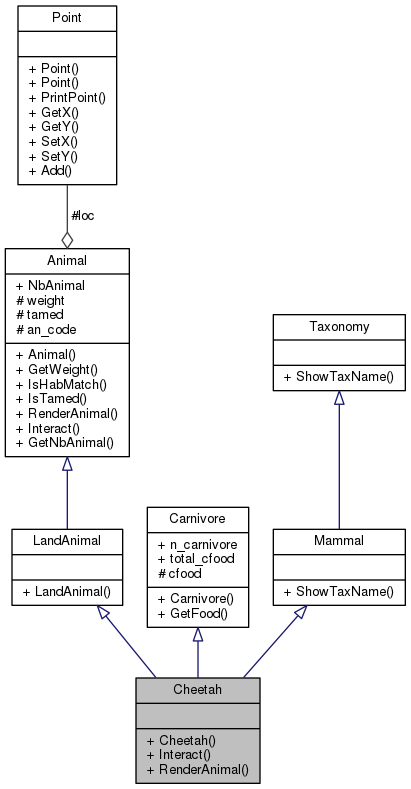
\includegraphics[width=224pt]{classCheetah__coll__graph}
\end{center}
\end{figure}
\subsection*{Public Member Functions}
\begin{DoxyCompactItemize}
\item 
\hyperlink{classCheetah_abfc6741349ff45ceb606ba5c128eb1e0}{Cheetah} (int x, int y)
\begin{DoxyCompactList}\small\item\em Constructor. \end{DoxyCompactList}\item 
void \hyperlink{classCheetah_aa7170571fd7285779257c86bc97cad93}{interact} ()\hypertarget{classCheetah_aa7170571fd7285779257c86bc97cad93}{}\label{classCheetah_aa7170571fd7285779257c86bc97cad93}

\begin{DoxyCompactList}\small\item\em Method interaksi cheetah. \end{DoxyCompactList}\end{DoxyCompactItemize}
\subsection*{Additional Inherited Members}


\subsection{Detailed Description}
Real class cheetah 

\subsection{Constructor \& Destructor Documentation}
\index{Cheetah@{Cheetah}!Cheetah@{Cheetah}}
\index{Cheetah@{Cheetah}!Cheetah@{Cheetah}}
\subsubsection[{\texorpdfstring{Cheetah(int x, int y)}{Cheetah(int x, int y)}}]{\setlength{\rightskip}{0pt plus 5cm}Cheetah\+::\+Cheetah (
\begin{DoxyParamCaption}
\item[{int}]{x, }
\item[{int}]{y}
\end{DoxyParamCaption}
)}\hypertarget{classCheetah_abfc6741349ff45ceb606ba5c128eb1e0}{}\label{classCheetah_abfc6741349ff45ceb606ba5c128eb1e0}


Constructor. 


\begin{DoxyParams}{Parameters}
{\em x} & absis lokasi \\
\hline
{\em y} & ordinat lokasi Konstruktor kelas cheetah \\
\hline
\end{DoxyParams}


The documentation for this class was generated from the following files\+:\begin{DoxyCompactItemize}
\item 
Land\+Animal.\+h\item 
Land\+Animal.\+cpp\end{DoxyCompactItemize}

\hypertarget{classChimpanzee}{}\section{Chimpanzee Class Reference}
\label{classChimpanzee}\index{Chimpanzee@{Chimpanzee}}


{\ttfamily \#include $<$Land\+Animal.\+h$>$}



Inheritance diagram for Chimpanzee\+:
\nopagebreak
\begin{figure}[H]
\begin{center}
\leavevmode
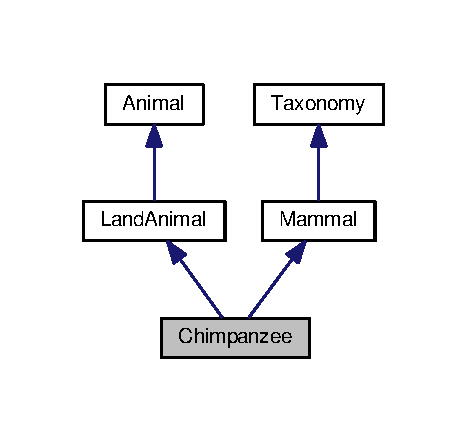
\includegraphics[width=224pt]{classChimpanzee__inherit__graph}
\end{center}
\end{figure}


Collaboration diagram for Chimpanzee\+:
\nopagebreak
\begin{figure}[H]
\begin{center}
\leavevmode
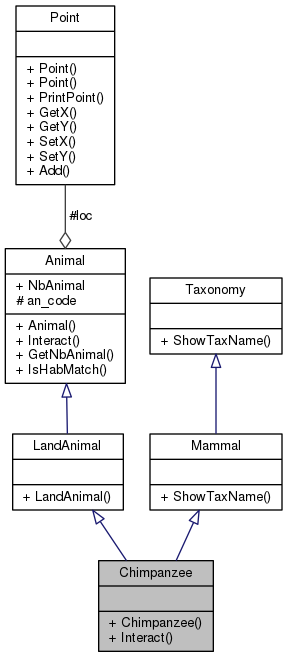
\includegraphics[width=224pt]{classChimpanzee__coll__graph}
\end{center}
\end{figure}
\subsection*{Public Member Functions}
\begin{DoxyCompactItemize}
\item 
\hyperlink{classChimpanzee_a11365fc4d031bf2895834721c060f0b3}{Chimpanzee} (int x, int y)
\begin{DoxyCompactList}\small\item\em Constructor. \end{DoxyCompactList}\item 
void \hyperlink{classChimpanzee_aade8161c7bcd697eae3d5a3559f6d976}{interact} ()\hypertarget{classChimpanzee_aade8161c7bcd697eae3d5a3559f6d976}{}\label{classChimpanzee_aade8161c7bcd697eae3d5a3559f6d976}

\begin{DoxyCompactList}\small\item\em Method interaksi chimpanzee. \end{DoxyCompactList}\end{DoxyCompactItemize}
\subsection*{Additional Inherited Members}


\subsection{Detailed Description}
Real class chimpanzee 

\subsection{Constructor \& Destructor Documentation}
\index{Chimpanzee@{Chimpanzee}!Chimpanzee@{Chimpanzee}}
\index{Chimpanzee@{Chimpanzee}!Chimpanzee@{Chimpanzee}}
\subsubsection[{\texorpdfstring{Chimpanzee(int x, int y)}{Chimpanzee(int x, int y)}}]{\setlength{\rightskip}{0pt plus 5cm}Chimpanzee\+::\+Chimpanzee (
\begin{DoxyParamCaption}
\item[{int}]{x, }
\item[{int}]{y}
\end{DoxyParamCaption}
)}\hypertarget{classChimpanzee_a11365fc4d031bf2895834721c060f0b3}{}\label{classChimpanzee_a11365fc4d031bf2895834721c060f0b3}


Constructor. 


\begin{DoxyParams}{Parameters}
{\em x} & absis lokasi \\
\hline
{\em y} & ordinat lokasi Konstruktor kelas chimpanzee \\
\hline
\end{DoxyParams}


The documentation for this class was generated from the following files\+:\begin{DoxyCompactItemize}
\item 
Land\+Animal.\+h\item 
Land\+Animal.\+cpp\end{DoxyCompactItemize}

\hypertarget{classCoala}{}\section{Coala Class Reference}
\label{classCoala}\index{Coala@{Coala}}


{\ttfamily \#include $<$Land\+Animal.\+h$>$}



Inheritance diagram for Coala\+:
% FIG 0


Collaboration diagram for Coala\+:
% FIG 1
\subsection*{Public Member Functions}
\begin{DoxyCompactItemize}
\item 
\hyperlink{classCoala_aad5c9bf3e235b775b21b5ffaf8d255f5}{Coala} (int x, int y)
\begin{DoxyCompactList}\small\item\em Constructor. \end{DoxyCompactList}\item 
void \hyperlink{classCoala_ad7d35de3f38bb1b708efec0a5c2c72a0}{interact} ()\hypertarget{classCoala_ad7d35de3f38bb1b708efec0a5c2c72a0}{}\label{classCoala_ad7d35de3f38bb1b708efec0a5c2c72a0}

\begin{DoxyCompactList}\small\item\em Method interaksi coala. \end{DoxyCompactList}\end{DoxyCompactItemize}
\subsection*{Additional Inherited Members}


\subsection{Detailed Description}
Real class coala 

\subsection{Constructor \& Destructor Documentation}
\index{Coala@{Coala}!Coala@{Coala}}
\index{Coala@{Coala}!Coala@{Coala}}
\subsubsection[{\texorpdfstring{Coala(int x, int y)}{Coala(int x, int y)}}]{\setlength{\rightskip}{0pt plus 5cm}Coala\+::\+Coala (
\begin{DoxyParamCaption}
\item[{int}]{x, }
\item[{int}]{y}
\end{DoxyParamCaption}
)}\hypertarget{classCoala_aad5c9bf3e235b775b21b5ffaf8d255f5}{}\label{classCoala_aad5c9bf3e235b775b21b5ffaf8d255f5}


Constructor. 


\begin{DoxyParams}{Parameters}
{\em x} & absis lokasi \\
\hline
{\em y} & ordinat lokasi Konstruktor kelas coala \\
\hline
\end{DoxyParams}


The documentation for this class was generated from the following files\+:\begin{DoxyCompactItemize}
\item 
Land\+Animal.\+h\item 
Land\+Animal.\+cpp\end{DoxyCompactItemize}

\hypertarget{classDolphin}{}\section{Dolphin Class Reference}
\label{classDolphin}\index{Dolphin@{Dolphin}}


{\ttfamily \#include $<$Water\+Animal.\+h$>$}



Inheritance diagram for Dolphin\+:
\nopagebreak
\begin{figure}[H]
\begin{center}
\leavevmode
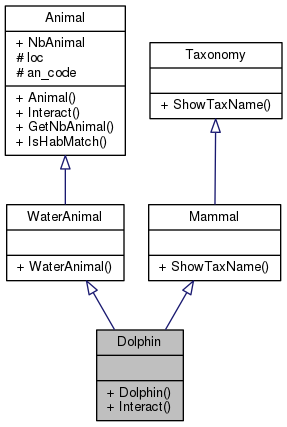
\includegraphics[width=230pt]{classDolphin__inherit__graph}
\end{center}
\end{figure}


Collaboration diagram for Dolphin\+:
\nopagebreak
\begin{figure}[H]
\begin{center}
\leavevmode
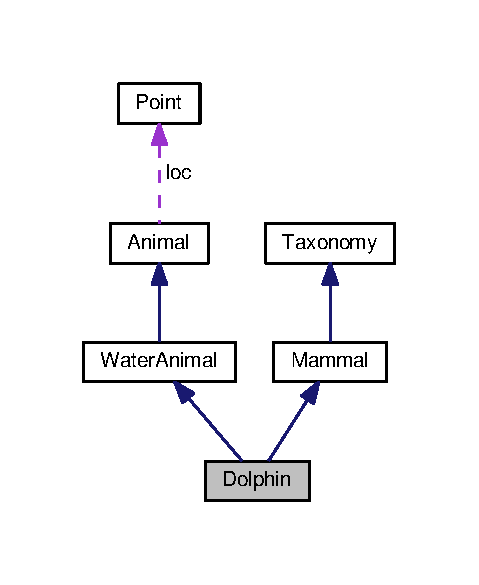
\includegraphics[width=230pt]{classDolphin__coll__graph}
\end{center}
\end{figure}
\subsection*{Public Member Functions}
\begin{DoxyCompactItemize}
\item 
\hyperlink{classDolphin_a7faed8c1c3a8dead1e28eef66bc1ac3c}{Dolphin} (int x, int y)
\begin{DoxyCompactList}\small\item\em Constructor. \end{DoxyCompactList}\item 
void \hyperlink{classDolphin_a6d5b202824f7f12e6286b2b09489c342}{interact} ()\hypertarget{classDolphin_a6d5b202824f7f12e6286b2b09489c342}{}\label{classDolphin_a6d5b202824f7f12e6286b2b09489c342}

\begin{DoxyCompactList}\small\item\em Method interaksi dolphin. \end{DoxyCompactList}\end{DoxyCompactItemize}
\subsection*{Additional Inherited Members}


\subsection{Detailed Description}
Real class dolphin 

\subsection{Constructor \& Destructor Documentation}
\index{Dolphin@{Dolphin}!Dolphin@{Dolphin}}
\index{Dolphin@{Dolphin}!Dolphin@{Dolphin}}
\subsubsection[{\texorpdfstring{Dolphin(int x, int y)}{Dolphin(int x, int y)}}]{\setlength{\rightskip}{0pt plus 5cm}Dolphin\+::\+Dolphin (
\begin{DoxyParamCaption}
\item[{int}]{x, }
\item[{int}]{y}
\end{DoxyParamCaption}
)}\hypertarget{classDolphin_a7faed8c1c3a8dead1e28eef66bc1ac3c}{}\label{classDolphin_a7faed8c1c3a8dead1e28eef66bc1ac3c}


Constructor. 


\begin{DoxyParams}{Parameters}
{\em x} & absis lokasi \\
\hline
{\em y} & ordinat lokasi Konstruktor kelas dolphin \\
\hline
\end{DoxyParams}


The documentation for this class was generated from the following files\+:\begin{DoxyCompactItemize}
\item 
Water\+Animal.\+h\item 
Water\+Animal.\+cpp\end{DoxyCompactItemize}

\hypertarget{classDriver}{}\section{Driver Class Reference}
\label{classDriver}\index{Driver@{Driver}}


Collaboration diagram for Driver\+:
% FIG 0
\subsection*{Public Member Functions}
\begin{DoxyCompactItemize}
\item 
{\bfseries Driver} (ifstream \&infile)\hypertarget{classDriver_a0cb90a693e4ef6a2365366a2eba715c0}{}\label{classDriver_a0cb90a693e4ef6a2365366a2eba715c0}

\item 
void {\bfseries Display\+Menu} ()\hypertarget{classDriver_a56f5ca7386659854399999ffb6d8d043}{}\label{classDriver_a56f5ca7386659854399999ffb6d8d043}

\item 
void {\bfseries Show\+Zoo} ()\hypertarget{classDriver_ad216c7b9cea5f8bc17b7951fe77e3cfd}{}\label{classDriver_ad216c7b9cea5f8bc17b7951fe77e3cfd}

\item 
void {\bfseries Tour\+Zoo} ()\hypertarget{classDriver_aa56ed0eaa789f78765708e15032d6534}{}\label{classDriver_aa56ed0eaa789f78765708e15032d6534}

\item 
void {\bfseries Animate\+Zoo} ()\hypertarget{classDriver_a18056fbf7b54a5210184c1c2383612cd}{}\label{classDriver_a18056fbf7b54a5210184c1c2383612cd}

\item 
void {\bfseries Food\+Zoo} ()\hypertarget{classDriver_ab5b75860466c7288d95f7344f3ce9991}{}\label{classDriver_ab5b75860466c7288d95f7344f3ce9991}

\item 
void {\bfseries Init\+Menu} ()\hypertarget{classDriver_a5083f9512c066cc061a021a76c1d3ec6}{}\label{classDriver_a5083f9512c066cc061a021a76c1d3ec6}

\item 
void {\bfseries Go\+To\+XY} (int x, int y)\hypertarget{classDriver_a04dc7a5d7be6e80e87e2de15bb6e648d}{}\label{classDriver_a04dc7a5d7be6e80e87e2de15bb6e648d}

\end{DoxyCompactItemize}


The documentation for this class was generated from the following files\+:\begin{DoxyCompactItemize}
\item 
driver/driver.\+h\item 
driver/driver.\+cpp\end{DoxyCompactItemize}

\hypertarget{classEagle}{}\section{Eagle Class Reference}
\label{classEagle}\index{Eagle@{Eagle}}


{\ttfamily \#include $<$Flying\+Animal.\+h$>$}



Inheritance diagram for Eagle\+:
\nopagebreak
\begin{figure}[H]
\begin{center}
\leavevmode
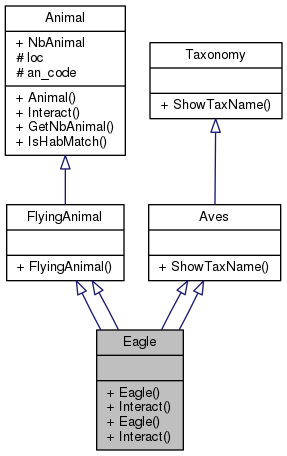
\includegraphics[width=222pt]{classEagle__inherit__graph}
\end{center}
\end{figure}


Collaboration diagram for Eagle\+:
\nopagebreak
\begin{figure}[H]
\begin{center}
\leavevmode
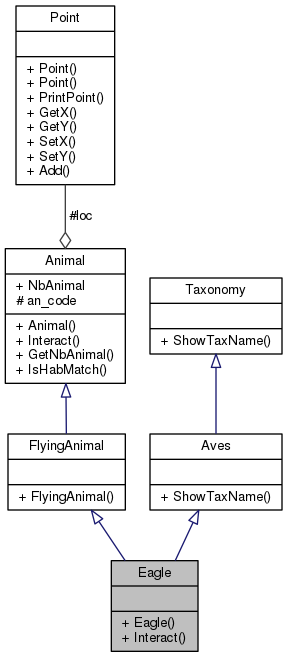
\includegraphics[width=222pt]{classEagle__coll__graph}
\end{center}
\end{figure}
\subsection*{Public Member Functions}
\begin{DoxyCompactItemize}
\item 
\hyperlink{classEagle_a8bb3b5bb543ecc9931ed47bc08a58a5a}{Eagle} (int x, int y)
\begin{DoxyCompactList}\small\item\em Constructor. \end{DoxyCompactList}\item 
void \hyperlink{classEagle_aa47ed62d92f1b2f9bad339b8521a50f6}{interact} ()\hypertarget{classEagle_aa47ed62d92f1b2f9bad339b8521a50f6}{}\label{classEagle_aa47ed62d92f1b2f9bad339b8521a50f6}

\begin{DoxyCompactList}\small\item\em Method interaksi eagle. \end{DoxyCompactList}\end{DoxyCompactItemize}
\subsection*{Additional Inherited Members}


\subsection{Detailed Description}
Real class eagle 

\subsection{Constructor \& Destructor Documentation}
\index{Eagle@{Eagle}!Eagle@{Eagle}}
\index{Eagle@{Eagle}!Eagle@{Eagle}}
\subsubsection[{\texorpdfstring{Eagle(int x, int y)}{Eagle(int x, int y)}}]{\setlength{\rightskip}{0pt plus 5cm}Eagle\+::\+Eagle (
\begin{DoxyParamCaption}
\item[{int}]{x, }
\item[{int}]{y}
\end{DoxyParamCaption}
)}\hypertarget{classEagle_a8bb3b5bb543ecc9931ed47bc08a58a5a}{}\label{classEagle_a8bb3b5bb543ecc9931ed47bc08a58a5a}


Constructor. 


\begin{DoxyParams}{Parameters}
{\em x} & absis lokasi \\
\hline
{\em y} & ordinat lokasi Konstruktor kelas eagle \\
\hline
\end{DoxyParams}


The documentation for this class was generated from the following files\+:\begin{DoxyCompactItemize}
\item 
Flying\+Animal.\+h\item 
Flying\+Animal.\+cpp\end{DoxyCompactItemize}

\hypertarget{classEntrance}{}\section{Entrance Class Reference}
\label{classEntrance}\index{Entrance@{Entrance}}


{\ttfamily \#include $<$Facility.\+h$>$}



Inheritance diagram for Entrance\+:
% FIG 0


Collaboration diagram for Entrance\+:
% FIG 1
\subsection*{Public Member Functions}
\begin{DoxyCompactItemize}
\item 
\hyperlink{classEntrance_acfb8b9f5d174b102562ee8989b8e20d4}{Entrance} (int x, int y)
\begin{DoxyCompactList}\small\item\em Constructor. \end{DoxyCompactList}\item 
void \hyperlink{classEntrance_afdd36c728c4ed589eed3e7bebb73d070}{render} ()\hypertarget{classEntrance_afdd36c728c4ed589eed3e7bebb73d070}{}\label{classEntrance_afdd36c728c4ed589eed3e7bebb73d070}

\begin{DoxyCompactList}\small\item\em Method render. \end{DoxyCompactList}\end{DoxyCompactItemize}
\subsection*{Additional Inherited Members}


\subsection{Detailed Description}
Real class entrance 

\subsection{Constructor \& Destructor Documentation}
\index{Entrance@{Entrance}!Entrance@{Entrance}}
\index{Entrance@{Entrance}!Entrance@{Entrance}}
\subsubsection[{\texorpdfstring{Entrance(int x, int y)}{Entrance(int x, int y)}}]{\setlength{\rightskip}{0pt plus 5cm}Entrance\+::\+Entrance (
\begin{DoxyParamCaption}
\item[{int}]{x, }
\item[{int}]{y}
\end{DoxyParamCaption}
)}\hypertarget{classEntrance_acfb8b9f5d174b102562ee8989b8e20d4}{}\label{classEntrance_acfb8b9f5d174b102562ee8989b8e20d4}


Constructor. 


\begin{DoxyParams}{Parameters}
{\em x} & absis lokasi \\
\hline
{\em y} & oridnat lokasi Konstruktor kelas entrance \\
\hline
\end{DoxyParams}


The documentation for this class was generated from the following files\+:\begin{DoxyCompactItemize}
\item 
Facility.\+h\item 
Facility.\+cpp\end{DoxyCompactItemize}

\hypertarget{classExit}{}\section{Exit Class Reference}
\label{classExit}\index{Exit@{Exit}}


{\ttfamily \#include $<$Facility.\+h$>$}



Inheritance diagram for Exit\+:
% FIG 0


Collaboration diagram for Exit\+:
% FIG 1
\subsection*{Public Member Functions}
\begin{DoxyCompactItemize}
\item 
\hyperlink{classExit_abb37d76b2e66fac8cac92fd61dfee563}{Exit} (int x, int y)
\begin{DoxyCompactList}\small\item\em Constructor. \end{DoxyCompactList}\item 
void \hyperlink{classExit_a7d8dae4579c58c28ab444de0fc4e62f5}{render} ()\hypertarget{classExit_a7d8dae4579c58c28ab444de0fc4e62f5}{}\label{classExit_a7d8dae4579c58c28ab444de0fc4e62f5}

\begin{DoxyCompactList}\small\item\em Method render. \end{DoxyCompactList}\end{DoxyCompactItemize}
\subsection*{Additional Inherited Members}


\subsection{Detailed Description}
Real class exit 

\subsection{Constructor \& Destructor Documentation}
\index{Exit@{Exit}!Exit@{Exit}}
\index{Exit@{Exit}!Exit@{Exit}}
\subsubsection[{\texorpdfstring{Exit(int x, int y)}{Exit(int x, int y)}}]{\setlength{\rightskip}{0pt plus 5cm}Exit\+::\+Exit (
\begin{DoxyParamCaption}
\item[{int}]{x, }
\item[{int}]{y}
\end{DoxyParamCaption}
)}\hypertarget{classExit_abb37d76b2e66fac8cac92fd61dfee563}{}\label{classExit_abb37d76b2e66fac8cac92fd61dfee563}


Constructor. 


\begin{DoxyParams}{Parameters}
{\em x} & absis lokasi \\
\hline
{\em y} & oridnat lokasi Konstruktor kelas exit \\
\hline
\end{DoxyParams}


The documentation for this class was generated from the following files\+:\begin{DoxyCompactItemize}
\item 
Facility.\+h\item 
Facility.\+cpp\end{DoxyCompactItemize}

\hypertarget{classFacility}{}\section{Facility Class Reference}
\label{classFacility}\index{Facility@{Facility}}


{\ttfamily \#include $<$facility.\+h$>$}



Inheritance diagram for Facility\+:
% FIG 0


Collaboration diagram for Facility\+:
% FIG 1
\subsection*{Public Member Functions}
\begin{DoxyCompactItemize}
\item 
\hyperlink{classFacility_aca76f1d74522884d7c9cfc742db5b9e3}{Facility} (int x, int y)
\begin{DoxyCompactList}\small\item\em Constructor. \end{DoxyCompactList}\end{DoxyCompactItemize}
\subsection*{Additional Inherited Members}


\subsection{Detailed Description}
Base class facility 

\subsection{Constructor \& Destructor Documentation}
\index{Facility@{Facility}!Facility@{Facility}}
\index{Facility@{Facility}!Facility@{Facility}}
\subsubsection[{\texorpdfstring{Facility(int x, int y)}{Facility(int x, int y)}}]{\setlength{\rightskip}{0pt plus 5cm}Facility\+::\+Facility (
\begin{DoxyParamCaption}
\item[{int}]{x, }
\item[{int}]{y}
\end{DoxyParamCaption}
)}\hypertarget{classFacility_aca76f1d74522884d7c9cfc742db5b9e3}{}\label{classFacility_aca76f1d74522884d7c9cfc742db5b9e3}


Constructor. 


\begin{DoxyParams}{Parameters}
{\em x} & absis lokasi \\
\hline
{\em y} & oridnat lokasi Konstruktor kelas facility \\
\hline
\end{DoxyParams}


The documentation for this class was generated from the following files\+:\begin{DoxyCompactItemize}
\item 
facility/facility.\+h\item 
facility/facility.\+cpp\end{DoxyCompactItemize}

\hypertarget{classFlyingAnimal}{}\section{Flying\+Animal Class Reference}
\label{classFlyingAnimal}\index{Flying\+Animal@{Flying\+Animal}}


Inheritance diagram for Flying\+Animal\+:
% FIG 0


Collaboration diagram for Flying\+Animal\+:
% FIG 1
\subsection*{Public Member Functions}
\begin{DoxyCompactItemize}
\item 
{\bfseries Flying\+Animal} (int x, int y)\hypertarget{classFlyingAnimal_a33fd442c27cb6f96404d274a69b44a9c}{}\label{classFlyingAnimal_a33fd442c27cb6f96404d274a69b44a9c}

\end{DoxyCompactItemize}
\subsection*{Additional Inherited Members}


The documentation for this class was generated from the following files\+:\begin{DoxyCompactItemize}
\item 
Animal.\+h\item 
Animal.\+cpp\end{DoxyCompactItemize}

\hypertarget{classFrog}{}\section{Frog Class Reference}
\label{classFrog}\index{Frog@{Frog}}


Inheritance diagram for Frog\+:
% FIG 0


Collaboration diagram for Frog\+:
% FIG 1
\subsection*{Public Member Functions}
\begin{DoxyCompactItemize}
\item 
\hyperlink{classFrog_a155019131b6ab65bab7bb97b538bdca5}{Frog} (int x, int y, int \hyperlink{classAnimal_a9a3b22f243f7109c57f36b3c660feb6e}{weight})
\begin{DoxyCompactList}\small\item\em Constructor. \end{DoxyCompactList}\item 
void \hyperlink{classFrog_aa6a785ec76a4123e3ec638029ed07f7f}{Interact} ()\hypertarget{classFrog_aa6a785ec76a4123e3ec638029ed07f7f}{}\label{classFrog_aa6a785ec76a4123e3ec638029ed07f7f}

\begin{DoxyCompactList}\small\item\em Method interaksi gorilla. \end{DoxyCompactList}\item 
void {\bfseries Render\+Animal} ()\hypertarget{classFrog_a8ac3be9660937d66bb5340aee6bbd402}{}\label{classFrog_a8ac3be9660937d66bb5340aee6bbd402}

\end{DoxyCompactItemize}
\subsection*{Additional Inherited Members}


\subsection{Constructor \& Destructor Documentation}
\index{Frog@{Frog}!Frog@{Frog}}
\index{Frog@{Frog}!Frog@{Frog}}
\subsubsection[{\texorpdfstring{Frog(int x, int y, int weight)}{Frog(int x, int y, int weight)}}]{\setlength{\rightskip}{0pt plus 5cm}Frog\+::\+Frog (
\begin{DoxyParamCaption}
\item[{int}]{x, }
\item[{int}]{y, }
\item[{int}]{weight}
\end{DoxyParamCaption}
)}\hypertarget{classFrog_a155019131b6ab65bab7bb97b538bdca5}{}\label{classFrog_a155019131b6ab65bab7bb97b538bdca5}


Constructor. 


\begin{DoxyParams}{Parameters}
{\em x} & absis lokasi \\
\hline
{\em y} & ordinat lokasi \\
\hline
{\em weight} & berat badan Konstruktor kelas gorilla \\
\hline
\end{DoxyParams}


The documentation for this class was generated from the following files\+:\begin{DoxyCompactItemize}
\item 
frog/frog.\+h\item 
frog/frog.\+cpp\end{DoxyCompactItemize}

\hypertarget{classGorilla}{}\section{Gorilla Class Reference}
\label{classGorilla}\index{Gorilla@{Gorilla}}


{\ttfamily \#include $<$Land\+Animal.\+h$>$}



Inheritance diagram for Gorilla\+:
% FIG 0


Collaboration diagram for Gorilla\+:
% FIG 1
\subsection*{Public Member Functions}
\begin{DoxyCompactItemize}
\item 
\hyperlink{classGorilla_addacb24475b69251ffab52377adb63fe}{Gorilla} (int x, int y)
\begin{DoxyCompactList}\small\item\em Constructor. \end{DoxyCompactList}\item 
void \hyperlink{classGorilla_ac0b08bebf807544f8821818986b26386}{interact} ()\hypertarget{classGorilla_ac0b08bebf807544f8821818986b26386}{}\label{classGorilla_ac0b08bebf807544f8821818986b26386}

\begin{DoxyCompactList}\small\item\em Method interaksi gorilla. \end{DoxyCompactList}\end{DoxyCompactItemize}
\subsection*{Additional Inherited Members}


\subsection{Detailed Description}
Real class gorilla 

\subsection{Constructor \& Destructor Documentation}
\index{Gorilla@{Gorilla}!Gorilla@{Gorilla}}
\index{Gorilla@{Gorilla}!Gorilla@{Gorilla}}
\subsubsection[{\texorpdfstring{Gorilla(int x, int y)}{Gorilla(int x, int y)}}]{\setlength{\rightskip}{0pt plus 5cm}Gorilla\+::\+Gorilla (
\begin{DoxyParamCaption}
\item[{int}]{x, }
\item[{int}]{y}
\end{DoxyParamCaption}
)}\hypertarget{classGorilla_addacb24475b69251ffab52377adb63fe}{}\label{classGorilla_addacb24475b69251ffab52377adb63fe}


Constructor. 


\begin{DoxyParams}{Parameters}
{\em x} & absis lokasi \\
\hline
{\em y} & ordinat lokasi Konstruktor kelas gorilla \\
\hline
\end{DoxyParams}


The documentation for this class was generated from the following files\+:\begin{DoxyCompactItemize}
\item 
Land\+Animal.\+h\item 
Land\+Animal.\+cpp\end{DoxyCompactItemize}

\hypertarget{classHabitat}{}\section{Habitat Class Reference}
\label{classHabitat}\index{Habitat@{Habitat}}


{\ttfamily \#include $<$Habitat.\+h$>$}



Inheritance diagram for Habitat\+:
\nopagebreak
\begin{figure}[H]
\begin{center}
\leavevmode
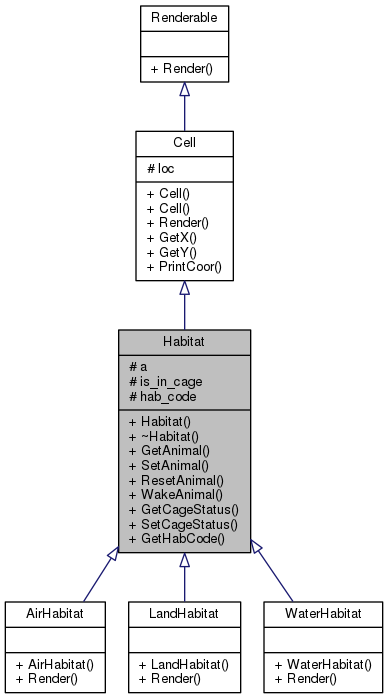
\includegraphics[width=320pt]{classHabitat__inherit__graph}
\end{center}
\end{figure}


Collaboration diagram for Habitat\+:
\nopagebreak
\begin{figure}[H]
\begin{center}
\leavevmode
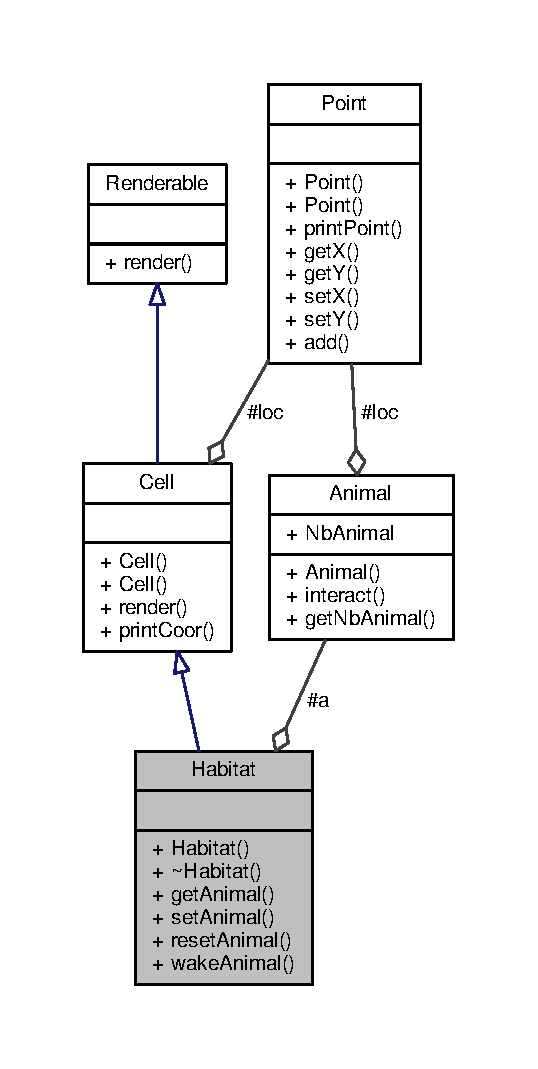
\includegraphics[width=209pt]{classHabitat__coll__graph}
\end{center}
\end{figure}
\subsection*{Public Member Functions}
\begin{DoxyCompactItemize}
\item 
\hyperlink{classHabitat_a7c44b3569efd42413f75b8dbc247f13d}{Habitat} (int x, int y)
\begin{DoxyCompactList}\small\item\em Constructor. \end{DoxyCompactList}\item 
\hyperlink{classAnimal}{Animal} $\ast$ {\bfseries get\+Animal} ()\hypertarget{classHabitat_adde39c6e68550831f7cf69333e6467c3}{}\label{classHabitat_adde39c6e68550831f7cf69333e6467c3}

\item 
void {\bfseries set\+Animal} (\hyperlink{classAnimal}{Animal} $\ast$an)\hypertarget{classHabitat_a1d721052c09f20e00c1719a3de9ce70a}{}\label{classHabitat_a1d721052c09f20e00c1719a3de9ce70a}

\item 
void {\bfseries reset\+Animal} ()\hypertarget{classHabitat_af7c572beb68a0d8b65c73331280fb9aa}{}\label{classHabitat_af7c572beb68a0d8b65c73331280fb9aa}

\item 
void {\bfseries wake\+Animal} ()\hypertarget{classHabitat_aafbf95dbb33f4555a037193b70e5336e}{}\label{classHabitat_aafbf95dbb33f4555a037193b70e5336e}

\end{DoxyCompactItemize}
\subsection*{Protected Attributes}
\begin{DoxyCompactItemize}
\item 
\hyperlink{classAnimal}{Animal} $\ast$ {\bfseries a}\hypertarget{classHabitat_a7ea1dfe236ddcd4121f186d75b33175a}{}\label{classHabitat_a7ea1dfe236ddcd4121f186d75b33175a}

\end{DoxyCompactItemize}


\subsection{Detailed Description}
A\+BC habitat 

\subsection{Constructor \& Destructor Documentation}
\index{Habitat@{Habitat}!Habitat@{Habitat}}
\index{Habitat@{Habitat}!Habitat@{Habitat}}
\subsubsection[{\texorpdfstring{Habitat(int x, int y)}{Habitat(int x, int y)}}]{\setlength{\rightskip}{0pt plus 5cm}Habitat\+::\+Habitat (
\begin{DoxyParamCaption}
\item[{int}]{x, }
\item[{int}]{y}
\end{DoxyParamCaption}
)}\hypertarget{classHabitat_a7c44b3569efd42413f75b8dbc247f13d}{}\label{classHabitat_a7c44b3569efd42413f75b8dbc247f13d}


Constructor. 


\begin{DoxyParams}{Parameters}
{\em x} & absis lokasi \\
\hline
{\em y} & oridnat lokasi Konstruktor kelas habitat \\
\hline
\end{DoxyParams}


The documentation for this class was generated from the following files\+:\begin{DoxyCompactItemize}
\item 
Habitat.\+h\item 
Habitat.\+cpp\end{DoxyCompactItemize}

\hypertarget{classHerbivore}{}\section{Herbivore Class Reference}
\label{classHerbivore}\index{Herbivore@{Herbivore}}


{\ttfamily \#include $<$herbivore.\+h$>$}



Inheritance diagram for Herbivore\+:
% FIG 0


Collaboration diagram for Herbivore\+:
% FIG 1
\subsection*{Public Member Functions}
\begin{DoxyCompactItemize}
\item 
\hyperlink{classHerbivore_a15f9af57f1d5d7eabb70fcc1619f1769}{Herbivore} (int weight)
\begin{DoxyCompactList}\small\item\em Constructor. \end{DoxyCompactList}\item 
float \hyperlink{classHerbivore_a2c63fd82a3919c52ca2d34c94d204ca4}{Get\+Food} () const \hypertarget{classHerbivore_a2c63fd82a3919c52ca2d34c94d204ca4}{}\label{classHerbivore_a2c63fd82a3919c52ca2d34c94d204ca4}

\begin{DoxyCompactList}\small\item\em Method Get\+Food mengembalikan makanan herbivora. \end{DoxyCompactList}\end{DoxyCompactItemize}
\subsection*{Static Public Attributes}
\begin{DoxyCompactItemize}
\item 
static int \hyperlink{classHerbivore_ad2c3c8409cb2b0c9f5fa1de7b9fd8430}{n\+\_\+herbivore} = 0
\item 
static float \hyperlink{classHerbivore_a8bd02e6119cd6950a37a8ef3e262fa0a}{total\+\_\+hfood} = 0
\end{DoxyCompactItemize}
\subsection*{Protected Attributes}
\begin{DoxyCompactItemize}
\item 
float \hyperlink{classHerbivore_a86962d379bc0fcc9b8921d8c39b333a7}{hfood}
\end{DoxyCompactItemize}


\subsection{Detailed Description}
Base class herbivore 

\subsection{Constructor \& Destructor Documentation}
\index{Herbivore@{Herbivore}!Herbivore@{Herbivore}}
\index{Herbivore@{Herbivore}!Herbivore@{Herbivore}}
\subsubsection[{\texorpdfstring{Herbivore(int weight)}{Herbivore(int weight)}}]{\setlength{\rightskip}{0pt plus 5cm}Herbivore\+::\+Herbivore (
\begin{DoxyParamCaption}
\item[{int}]{weight}
\end{DoxyParamCaption}
)}\hypertarget{classHerbivore_a15f9af57f1d5d7eabb70fcc1619f1769}{}\label{classHerbivore_a15f9af57f1d5d7eabb70fcc1619f1769}


Constructor. 


\begin{DoxyParams}{Parameters}
{\em weight} & Konstruktor herbivore dengan parameter berat badan \\
\hline
\end{DoxyParams}


\subsection{Member Data Documentation}
\index{Herbivore@{Herbivore}!hfood@{hfood}}
\index{hfood@{hfood}!Herbivore@{Herbivore}}
\subsubsection[{\texorpdfstring{hfood}{hfood}}]{\setlength{\rightskip}{0pt plus 5cm}float Herbivore\+::hfood\hspace{0.3cm}{\ttfamily [protected]}}\hypertarget{classHerbivore_a86962d379bc0fcc9b8921d8c39b333a7}{}\label{classHerbivore_a86962d379bc0fcc9b8921d8c39b333a7}
Makanan herbivora \index{Herbivore@{Herbivore}!n\+\_\+herbivore@{n\+\_\+herbivore}}
\index{n\+\_\+herbivore@{n\+\_\+herbivore}!Herbivore@{Herbivore}}
\subsubsection[{\texorpdfstring{n\+\_\+herbivore}{n_herbivore}}]{\setlength{\rightskip}{0pt plus 5cm}int Herbivore\+::n\+\_\+herbivore = 0\hspace{0.3cm}{\ttfamily [static]}}\hypertarget{classHerbivore_ad2c3c8409cb2b0c9f5fa1de7b9fd8430}{}\label{classHerbivore_ad2c3c8409cb2b0c9f5fa1de7b9fd8430}
Jumlah hewan herbivora \index{Herbivore@{Herbivore}!total\+\_\+hfood@{total\+\_\+hfood}}
\index{total\+\_\+hfood@{total\+\_\+hfood}!Herbivore@{Herbivore}}
\subsubsection[{\texorpdfstring{total\+\_\+hfood}{total_hfood}}]{\setlength{\rightskip}{0pt plus 5cm}float Herbivore\+::total\+\_\+hfood = 0\hspace{0.3cm}{\ttfamily [static]}}\hypertarget{classHerbivore_a8bd02e6119cd6950a37a8ef3e262fa0a}{}\label{classHerbivore_a8bd02e6119cd6950a37a8ef3e262fa0a}
Jumlah total makanan herbivora 

The documentation for this class was generated from the following files\+:\begin{DoxyCompactItemize}
\item 
herbivore/herbivore.\+h\item 
herbivore/herbivore.\+cpp\end{DoxyCompactItemize}

\hypertarget{classHyena}{}\section{Hyena Class Reference}
\label{classHyena}\index{Hyena@{Hyena}}


{\ttfamily \#include $<$Land\+Animal.\+h$>$}



Inheritance diagram for Hyena\+:
\nopagebreak
\begin{figure}[H]
\begin{center}
\leavevmode
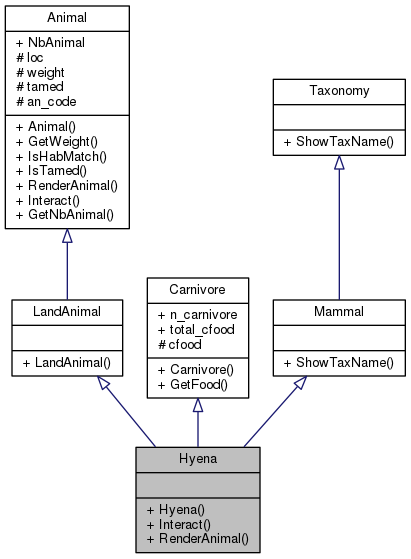
\includegraphics[width=224pt]{classHyena__inherit__graph}
\end{center}
\end{figure}


Collaboration diagram for Hyena\+:
\nopagebreak
\begin{figure}[H]
\begin{center}
\leavevmode
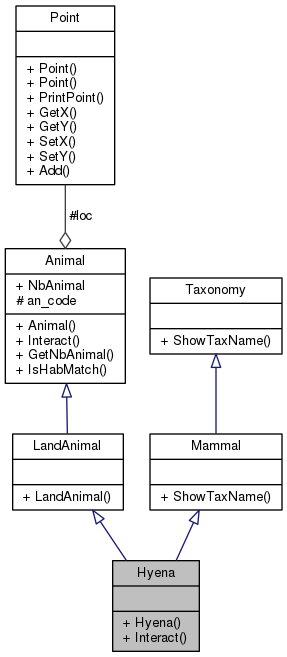
\includegraphics[width=224pt]{classHyena__coll__graph}
\end{center}
\end{figure}
\subsection*{Public Member Functions}
\begin{DoxyCompactItemize}
\item 
\hyperlink{classHyena_a49a9c409606187720e4fbde4b248f1e6}{Hyena} (int x, int y)
\begin{DoxyCompactList}\small\item\em Constructor. \end{DoxyCompactList}\item 
void \hyperlink{classHyena_aaac9f93962c49ea129626bc7719bcbe7}{interact} ()\hypertarget{classHyena_aaac9f93962c49ea129626bc7719bcbe7}{}\label{classHyena_aaac9f93962c49ea129626bc7719bcbe7}

\begin{DoxyCompactList}\small\item\em Method interaksi hyena. \end{DoxyCompactList}\end{DoxyCompactItemize}
\subsection*{Additional Inherited Members}


\subsection{Detailed Description}
Real class hyena 

\subsection{Constructor \& Destructor Documentation}
\index{Hyena@{Hyena}!Hyena@{Hyena}}
\index{Hyena@{Hyena}!Hyena@{Hyena}}
\subsubsection[{\texorpdfstring{Hyena(int x, int y)}{Hyena(int x, int y)}}]{\setlength{\rightskip}{0pt plus 5cm}Hyena\+::\+Hyena (
\begin{DoxyParamCaption}
\item[{int}]{x, }
\item[{int}]{y}
\end{DoxyParamCaption}
)}\hypertarget{classHyena_a49a9c409606187720e4fbde4b248f1e6}{}\label{classHyena_a49a9c409606187720e4fbde4b248f1e6}


Constructor. 


\begin{DoxyParams}{Parameters}
{\em x} & absis lokasi \\
\hline
{\em y} & ordinat lokasi Konstruktor kelas hyena \\
\hline
\end{DoxyParams}


The documentation for this class was generated from the following files\+:\begin{DoxyCompactItemize}
\item 
Land\+Animal.\+h\item 
Land\+Animal.\+cpp\end{DoxyCompactItemize}

\hypertarget{classKangaroo}{}\section{Kangaroo Class Reference}
\label{classKangaroo}\index{Kangaroo@{Kangaroo}}


{\ttfamily \#include $<$Land\+Animal.\+h$>$}



Inheritance diagram for Kangaroo\+:
\nopagebreak
\begin{figure}[H]
\begin{center}
\leavevmode
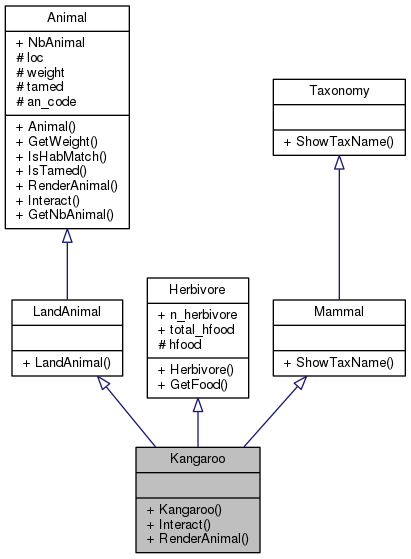
\includegraphics[width=224pt]{classKangaroo__inherit__graph}
\end{center}
\end{figure}


Collaboration diagram for Kangaroo\+:
\nopagebreak
\begin{figure}[H]
\begin{center}
\leavevmode
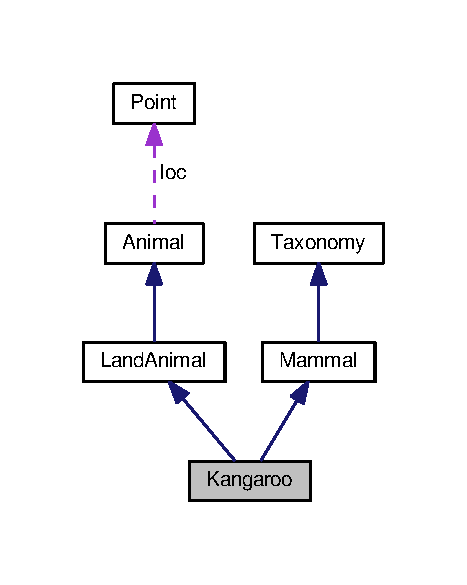
\includegraphics[width=224pt]{classKangaroo__coll__graph}
\end{center}
\end{figure}
\subsection*{Public Member Functions}
\begin{DoxyCompactItemize}
\item 
\hyperlink{classKangaroo_a051c76596036d0cf2a29ff8acb24209e}{Kangaroo} (int x, int y)
\begin{DoxyCompactList}\small\item\em Constructor. \end{DoxyCompactList}\item 
void \hyperlink{classKangaroo_afe7cdf7299c0afeb73e5e43c0bf77105}{interact} ()\hypertarget{classKangaroo_afe7cdf7299c0afeb73e5e43c0bf77105}{}\label{classKangaroo_afe7cdf7299c0afeb73e5e43c0bf77105}

\begin{DoxyCompactList}\small\item\em Method interaksi kangaroo. \end{DoxyCompactList}\end{DoxyCompactItemize}
\subsection*{Additional Inherited Members}


\subsection{Detailed Description}
Real class kangaroo 

\subsection{Constructor \& Destructor Documentation}
\index{Kangaroo@{Kangaroo}!Kangaroo@{Kangaroo}}
\index{Kangaroo@{Kangaroo}!Kangaroo@{Kangaroo}}
\subsubsection[{\texorpdfstring{Kangaroo(int x, int y)}{Kangaroo(int x, int y)}}]{\setlength{\rightskip}{0pt plus 5cm}Kangaroo\+::\+Kangaroo (
\begin{DoxyParamCaption}
\item[{int}]{x, }
\item[{int}]{y}
\end{DoxyParamCaption}
)}\hypertarget{classKangaroo_a051c76596036d0cf2a29ff8acb24209e}{}\label{classKangaroo_a051c76596036d0cf2a29ff8acb24209e}


Constructor. 


\begin{DoxyParams}{Parameters}
{\em x} & absis lokasi \\
\hline
{\em y} & ordinat lokasi Konstruktor kelas kangaroo \\
\hline
\end{DoxyParams}


The documentation for this class was generated from the following files\+:\begin{DoxyCompactItemize}
\item 
Land\+Animal.\+h\item 
Land\+Animal.\+cpp\end{DoxyCompactItemize}

\hypertarget{classKolibri}{}\section{Kolibri Class Reference}
\label{classKolibri}\index{Kolibri@{Kolibri}}


{\ttfamily \#include $<$Flying\+Animal.\+h$>$}



Inheritance diagram for Kolibri\+:
% FIG 0


Collaboration diagram for Kolibri\+:
% FIG 1
\subsection*{Public Member Functions}
\begin{DoxyCompactItemize}
\item 
\hyperlink{classKolibri_ae4af707d315c614de90cd7be073215f9}{Kolibri} (int x, int y)
\begin{DoxyCompactList}\small\item\em Constructor. \end{DoxyCompactList}\item 
void \hyperlink{classKolibri_aea697342d51b3946dfcf07ab905492a6}{interact} ()\hypertarget{classKolibri_aea697342d51b3946dfcf07ab905492a6}{}\label{classKolibri_aea697342d51b3946dfcf07ab905492a6}

\begin{DoxyCompactList}\small\item\em Method interaksi kolibri. \end{DoxyCompactList}\end{DoxyCompactItemize}
\subsection*{Additional Inherited Members}


\subsection{Detailed Description}
Real class kolibri 

\subsection{Constructor \& Destructor Documentation}
\index{Kolibri@{Kolibri}!Kolibri@{Kolibri}}
\index{Kolibri@{Kolibri}!Kolibri@{Kolibri}}
\subsubsection[{\texorpdfstring{Kolibri(int x, int y)}{Kolibri(int x, int y)}}]{\setlength{\rightskip}{0pt plus 5cm}Kolibri\+::\+Kolibri (
\begin{DoxyParamCaption}
\item[{int}]{x, }
\item[{int}]{y}
\end{DoxyParamCaption}
)}\hypertarget{classKolibri_ae4af707d315c614de90cd7be073215f9}{}\label{classKolibri_ae4af707d315c614de90cd7be073215f9}


Constructor. 


\begin{DoxyParams}{Parameters}
{\em x} & absis lokasi \\
\hline
{\em y} & ordinat lokasi Konstruktor kelas kolibri \\
\hline
\end{DoxyParams}


The documentation for this class was generated from the following files\+:\begin{DoxyCompactItemize}
\item 
Flying\+Animal.\+h\item 
Flying\+Animal.\+cpp\end{DoxyCompactItemize}

\hypertarget{classKomodo}{}\section{Komodo Class Reference}
\label{classKomodo}\index{Komodo@{Komodo}}


{\ttfamily \#include $<$komodo.\+h$>$}



Inheritance diagram for Komodo\+:
% FIG 0


Collaboration diagram for Komodo\+:
% FIG 1
\subsection*{Public Member Functions}
\begin{DoxyCompactItemize}
\item 
\hyperlink{classKomodo_aa040951c2340068812bb513d87948947}{Komodo} (int x, int y, int \hyperlink{classAnimal_a9a3b22f243f7109c57f36b3c660feb6e}{weight})
\begin{DoxyCompactList}\small\item\em Constructor. \end{DoxyCompactList}\item 
void \hyperlink{classKomodo_ab3b3b931d96321b809f6db8c04f2dc77}{Interact} ()\hypertarget{classKomodo_ab3b3b931d96321b809f6db8c04f2dc77}{}\label{classKomodo_ab3b3b931d96321b809f6db8c04f2dc77}

\begin{DoxyCompactList}\small\item\em Method interaksi komodo. \end{DoxyCompactList}\item 
void {\bfseries Render\+Animal} ()\hypertarget{classKomodo_ae34363afb6c2505ae1a03fa32f9a8c8a}{}\label{classKomodo_ae34363afb6c2505ae1a03fa32f9a8c8a}

\end{DoxyCompactItemize}
\subsection*{Additional Inherited Members}


\subsection{Detailed Description}
Real class komodo 

\subsection{Constructor \& Destructor Documentation}
\index{Komodo@{Komodo}!Komodo@{Komodo}}
\index{Komodo@{Komodo}!Komodo@{Komodo}}
\subsubsection[{\texorpdfstring{Komodo(int x, int y, int weight)}{Komodo(int x, int y, int weight)}}]{\setlength{\rightskip}{0pt plus 5cm}Komodo\+::\+Komodo (
\begin{DoxyParamCaption}
\item[{int}]{x, }
\item[{int}]{y, }
\item[{int}]{weight}
\end{DoxyParamCaption}
)}\hypertarget{classKomodo_aa040951c2340068812bb513d87948947}{}\label{classKomodo_aa040951c2340068812bb513d87948947}


Constructor. 


\begin{DoxyParams}{Parameters}
{\em x} & absis lokasi \\
\hline
{\em y} & ordinat lokasi \\
\hline
{\em weight} & berat badan Konstruktor kelas komodo \\
\hline
\end{DoxyParams}


The documentation for this class was generated from the following files\+:\begin{DoxyCompactItemize}
\item 
komodo/komodo.\+h\item 
komodo/komodo.\+cpp\end{DoxyCompactItemize}

\hypertarget{classLandAnimal}{}\section{Land\+Animal Class Reference}
\label{classLandAnimal}\index{Land\+Animal@{Land\+Animal}}


Inheritance diagram for Land\+Animal\+:
\nopagebreak
\begin{figure}[H]
\begin{center}
\leavevmode
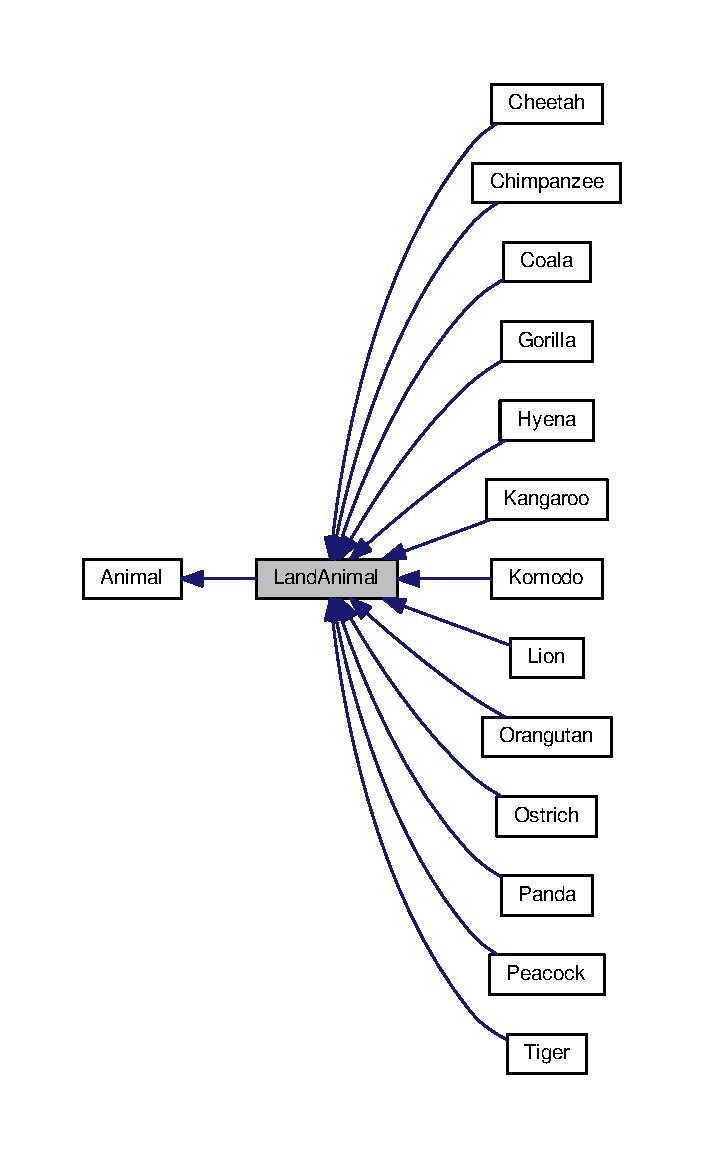
\includegraphics[width=350pt]{classLandAnimal__inherit__graph}
\end{center}
\end{figure}


Collaboration diagram for Land\+Animal\+:
\nopagebreak
\begin{figure}[H]
\begin{center}
\leavevmode
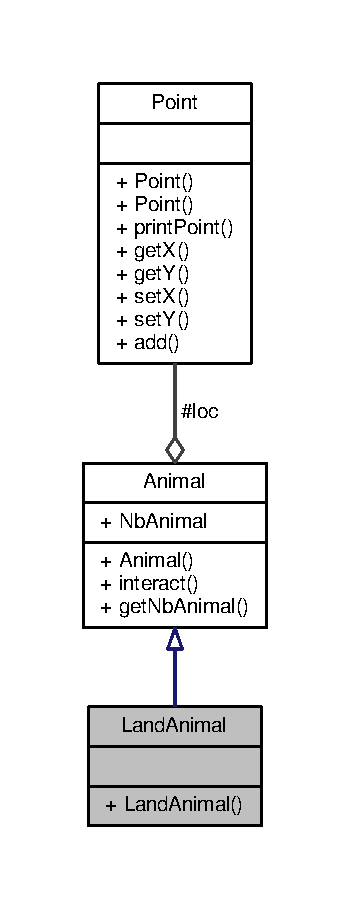
\includegraphics[width=168pt]{classLandAnimal__coll__graph}
\end{center}
\end{figure}
\subsection*{Public Member Functions}
\begin{DoxyCompactItemize}
\item 
{\bfseries Land\+Animal} (int x, int y)\hypertarget{classLandAnimal_a93384d0797a56eac2e276b8b2f5cd4f1}{}\label{classLandAnimal_a93384d0797a56eac2e276b8b2f5cd4f1}

\end{DoxyCompactItemize}
\subsection*{Additional Inherited Members}


The documentation for this class was generated from the following files\+:\begin{DoxyCompactItemize}
\item 
Animal.\+h\item 
Animal.\+cpp\end{DoxyCompactItemize}

\hypertarget{classLandHabitat}{}\section{Land\+Habitat Class Reference}
\label{classLandHabitat}\index{Land\+Habitat@{Land\+Habitat}}


{\ttfamily \#include $<$Habitat.\+h$>$}



Inheritance diagram for Land\+Habitat\+:
\nopagebreak
\begin{figure}[H]
\begin{center}
\leavevmode
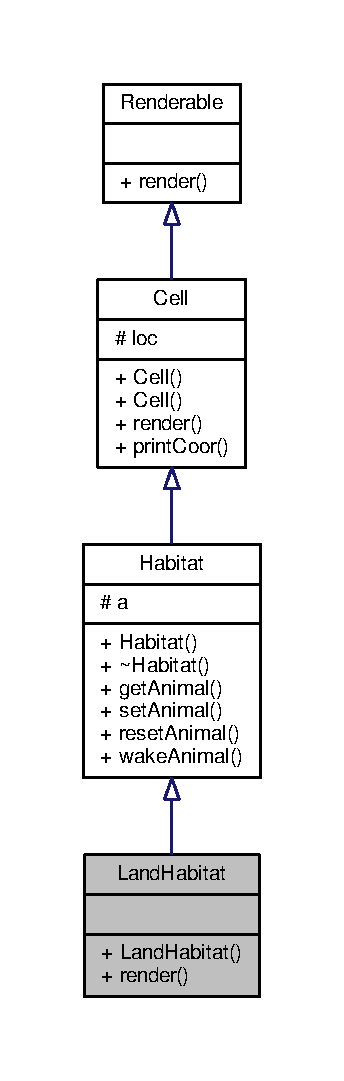
\includegraphics[width=149pt]{classLandHabitat__inherit__graph}
\end{center}
\end{figure}


Collaboration diagram for Land\+Habitat\+:
\nopagebreak
\begin{figure}[H]
\begin{center}
\leavevmode
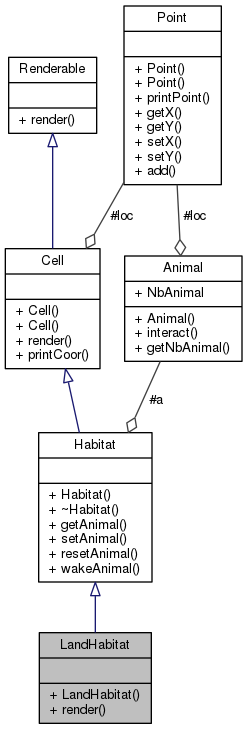
\includegraphics[width=209pt]{classLandHabitat__coll__graph}
\end{center}
\end{figure}
\subsection*{Public Member Functions}
\begin{DoxyCompactItemize}
\item 
{\bfseries Land\+Habitat} (int x, int y)\hypertarget{classLandHabitat_a2ca94610d493f3bd8b54b3b53a231536}{}\label{classLandHabitat_a2ca94610d493f3bd8b54b3b53a231536}

\item 
void \hyperlink{classLandHabitat_ad90a2fd22fa5b521d5e19e61798e3175}{render} ()\hypertarget{classLandHabitat_ad90a2fd22fa5b521d5e19e61798e3175}{}\label{classLandHabitat_ad90a2fd22fa5b521d5e19e61798e3175}

\begin{DoxyCompactList}\small\item\em Method render. \end{DoxyCompactList}\end{DoxyCompactItemize}
\subsection*{Additional Inherited Members}


\subsection{Detailed Description}
Base class landhabitat


\begin{DoxyParams}{Parameters}
{\em x} & absis lokasi \\
\hline
{\em y} & oridnat lokasi Konstruktor landhabitat \\
\hline
\end{DoxyParams}


The documentation for this class was generated from the following files\+:\begin{DoxyCompactItemize}
\item 
Habitat.\+h\item 
Habitat.\+cpp\end{DoxyCompactItemize}

\hypertarget{classLandWaterAnimal}{}\section{Land\+Water\+Animal Class Reference}
\label{classLandWaterAnimal}\index{Land\+Water\+Animal@{Land\+Water\+Animal}}


Inheritance diagram for Land\+Water\+Animal\+:
% FIG 0


Collaboration diagram for Land\+Water\+Animal\+:
% FIG 1
\subsection*{Public Member Functions}
\begin{DoxyCompactItemize}
\item 
{\bfseries Land\+Water\+Animal} (int x, int y, int w)\hypertarget{classLandWaterAnimal_adef93b8ab6ece0bf9c12a53569c4c794}{}\label{classLandWaterAnimal_adef93b8ab6ece0bf9c12a53569c4c794}

\end{DoxyCompactItemize}
\subsection*{Additional Inherited Members}


The documentation for this class was generated from the following files\+:\begin{DoxyCompactItemize}
\item 
land\+\_\+water\+\_\+animal/land\+\_\+water\+\_\+animal.\+h\item 
land\+\_\+water\+\_\+animal/land\+\_\+water\+\_\+animal.\+cpp\end{DoxyCompactItemize}

\hypertarget{classLion}{}\section{Lion Class Reference}
\label{classLion}\index{Lion@{Lion}}


{\ttfamily \#include $<$Land\+Animal.\+h$>$}



Inheritance diagram for Lion\+:
% FIG 0


Collaboration diagram for Lion\+:
% FIG 1
\subsection*{Public Member Functions}
\begin{DoxyCompactItemize}
\item 
\hyperlink{classLion_a225819c524decec8694b1c651923aa5f}{Lion} (int x, int y)
\begin{DoxyCompactList}\small\item\em Constructor. \end{DoxyCompactList}\item 
void \hyperlink{classLion_a4e12205d48a96d7cc32c8fa45cd1f5e0}{interact} ()\hypertarget{classLion_a4e12205d48a96d7cc32c8fa45cd1f5e0}{}\label{classLion_a4e12205d48a96d7cc32c8fa45cd1f5e0}

\begin{DoxyCompactList}\small\item\em Method interaksi lion. \end{DoxyCompactList}\end{DoxyCompactItemize}
\subsection*{Additional Inherited Members}


\subsection{Detailed Description}
Real class lion 

\subsection{Constructor \& Destructor Documentation}
\index{Lion@{Lion}!Lion@{Lion}}
\index{Lion@{Lion}!Lion@{Lion}}
\subsubsection[{\texorpdfstring{Lion(int x, int y)}{Lion(int x, int y)}}]{\setlength{\rightskip}{0pt plus 5cm}Lion\+::\+Lion (
\begin{DoxyParamCaption}
\item[{int}]{x, }
\item[{int}]{y}
\end{DoxyParamCaption}
)}\hypertarget{classLion_a225819c524decec8694b1c651923aa5f}{}\label{classLion_a225819c524decec8694b1c651923aa5f}


Constructor. 


\begin{DoxyParams}{Parameters}
{\em x} & absis lokasi \\
\hline
{\em y} & ordinat lokasi Konstruktor kelas lion \\
\hline
\end{DoxyParams}


The documentation for this class was generated from the following files\+:\begin{DoxyCompactItemize}
\item 
Land\+Animal.\+h\item 
Land\+Animal.\+cpp\end{DoxyCompactItemize}

\hypertarget{classMammal}{}\section{Mammal Class Reference}
\label{classMammal}\index{Mammal@{Mammal}}


{\ttfamily \#include $<$Taxonomy.\+h$>$}



Inheritance diagram for Mammal\+:
\nopagebreak
\begin{figure}[H]
\begin{center}
\leavevmode
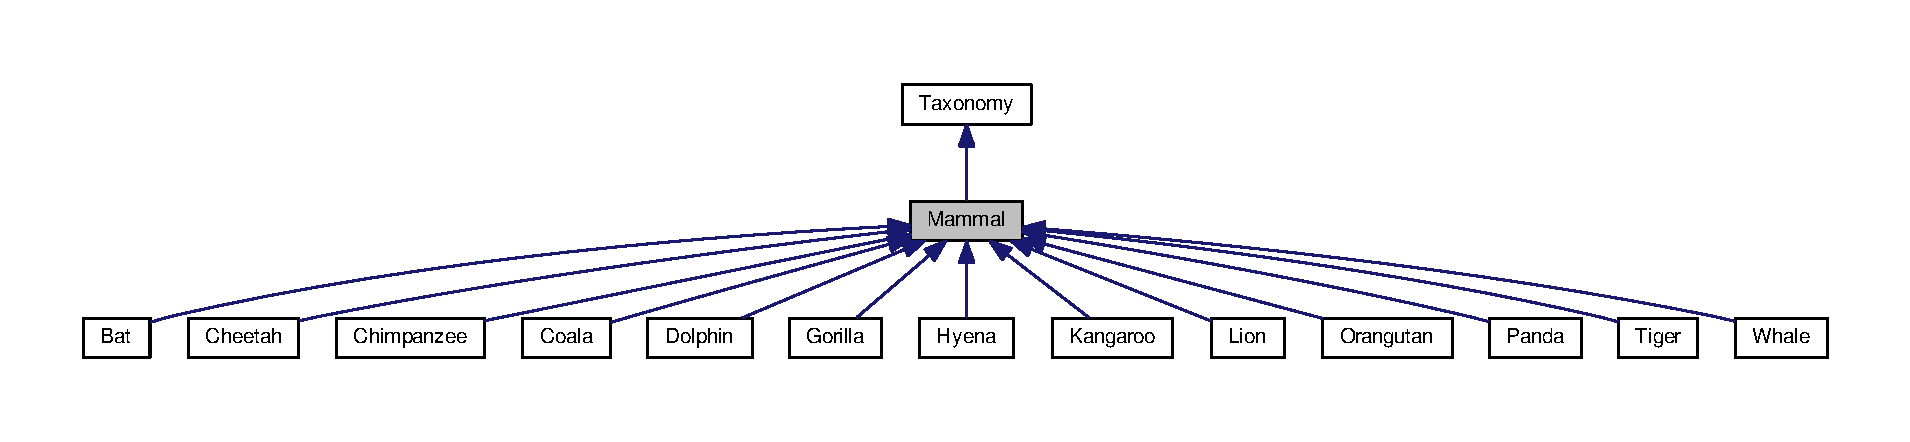
\includegraphics[width=350pt]{classMammal__inherit__graph}
\end{center}
\end{figure}


Collaboration diagram for Mammal\+:
\nopagebreak
\begin{figure}[H]
\begin{center}
\leavevmode
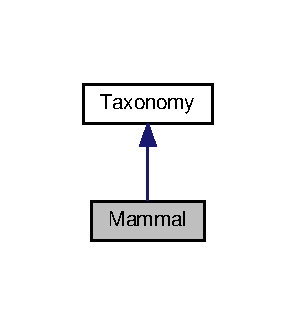
\includegraphics[width=178pt]{classMammal__coll__graph}
\end{center}
\end{figure}
\subsection*{Public Member Functions}
\begin{DoxyCompactItemize}
\item 
void \hyperlink{classMammal_a339b8cfa7a68fd1df89bce06c24e62ff}{show\+Tax\+Name} ()\hypertarget{classMammal_a339b8cfa7a68fd1df89bce06c24e62ff}{}\label{classMammal_a339b8cfa7a68fd1df89bce06c24e62ff}

\begin{DoxyCompactList}\small\item\em method show\+Name. Menampilkan nama taksonomi. \end{DoxyCompactList}\end{DoxyCompactItemize}


\subsection{Detailed Description}
Base class 

The documentation for this class was generated from the following files\+:\begin{DoxyCompactItemize}
\item 
Taxonomy.\+h\item 
Taxonomy.\+cpp\end{DoxyCompactItemize}

\hypertarget{classMantaray}{}\section{Mantaray Class Reference}
\label{classMantaray}\index{Mantaray@{Mantaray}}


{\ttfamily \#include $<$Water\+Animal.\+h$>$}



Inheritance diagram for Mantaray\+:
\nopagebreak
\begin{figure}[H]
\begin{center}
\leavevmode
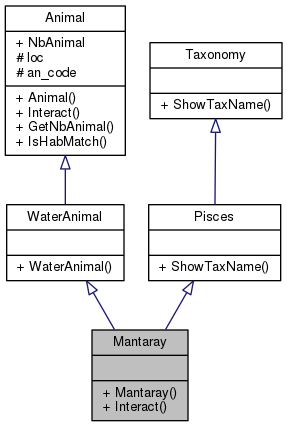
\includegraphics[width=284pt]{classMantaray__inherit__graph}
\end{center}
\end{figure}


Collaboration diagram for Mantaray\+:
\nopagebreak
\begin{figure}[H]
\begin{center}
\leavevmode
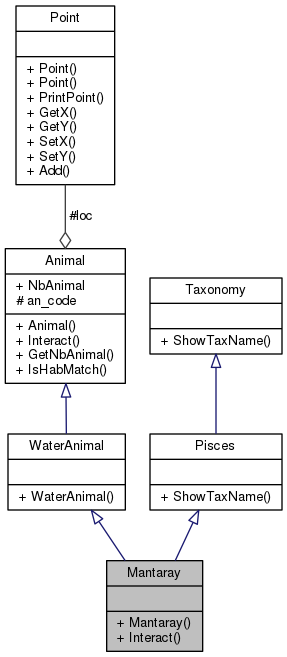
\includegraphics[width=284pt]{classMantaray__coll__graph}
\end{center}
\end{figure}
\subsection*{Public Member Functions}
\begin{DoxyCompactItemize}
\item 
\hyperlink{classMantaray_abc2e69b76fb33a0e121e894e1d96352c}{Mantaray} (int x, int y)
\begin{DoxyCompactList}\small\item\em Constructor. \end{DoxyCompactList}\item 
void \hyperlink{classMantaray_ac6a64db1f04b43eec33887e625dd6761}{interact} ()\hypertarget{classMantaray_ac6a64db1f04b43eec33887e625dd6761}{}\label{classMantaray_ac6a64db1f04b43eec33887e625dd6761}

\begin{DoxyCompactList}\small\item\em Method interaksi mantaray. \end{DoxyCompactList}\end{DoxyCompactItemize}
\subsection*{Additional Inherited Members}


\subsection{Detailed Description}
Real class mantaray 

\subsection{Constructor \& Destructor Documentation}
\index{Mantaray@{Mantaray}!Mantaray@{Mantaray}}
\index{Mantaray@{Mantaray}!Mantaray@{Mantaray}}
\subsubsection[{\texorpdfstring{Mantaray(int x, int y)}{Mantaray(int x, int y)}}]{\setlength{\rightskip}{0pt plus 5cm}Mantaray\+::\+Mantaray (
\begin{DoxyParamCaption}
\item[{int}]{x, }
\item[{int}]{y}
\end{DoxyParamCaption}
)}\hypertarget{classMantaray_abc2e69b76fb33a0e121e894e1d96352c}{}\label{classMantaray_abc2e69b76fb33a0e121e894e1d96352c}


Constructor. 


\begin{DoxyParams}{Parameters}
{\em x} & absis lokasi \\
\hline
{\em y} & ordinat lokasi Konstruktor kelas mantaray \\
\hline
\end{DoxyParams}


The documentation for this class was generated from the following files\+:\begin{DoxyCompactItemize}
\item 
Water\+Animal.\+h\item 
Water\+Animal.\+cpp\end{DoxyCompactItemize}

\hypertarget{classOmnivore}{}\section{Omnivore Class Reference}
\label{classOmnivore}\index{Omnivore@{Omnivore}}


{\ttfamily \#include $<$omnivore.\+h$>$}



Inheritance diagram for Omnivore\+:
% FIG 0


Collaboration diagram for Omnivore\+:
% FIG 1
\subsection*{Public Member Functions}
\begin{DoxyCompactItemize}
\item 
\hyperlink{classOmnivore_a8e20388c09d013115ebe629c8e5b027a}{Omnivore} (int weight)
\begin{DoxyCompactList}\small\item\em Constructor. \end{DoxyCompactList}\item 
float \hyperlink{classOmnivore_a701d76169b7ac6581fa4b9434902f04b}{Get\+Food} () const \hypertarget{classOmnivore_a701d76169b7ac6581fa4b9434902f04b}{}\label{classOmnivore_a701d76169b7ac6581fa4b9434902f04b}

\begin{DoxyCompactList}\small\item\em Method Get\+Food mengembalikan makanan omnivora. \end{DoxyCompactList}\end{DoxyCompactItemize}
\subsection*{Static Public Attributes}
\begin{DoxyCompactItemize}
\item 
static int \hyperlink{classOmnivore_ab625c981d2a5a3c2e6f72fae17ea0bf0}{n\+\_\+omnivore} = 0
\item 
static float \hyperlink{classOmnivore_ac4e106c20ef52747fb78f22765beaa64}{total\+\_\+ofood} = 0
\end{DoxyCompactItemize}
\subsection*{Protected Attributes}
\begin{DoxyCompactItemize}
\item 
float \hyperlink{classOmnivore_a71b234f7a70601f96a92c3a16d373d17}{ofood}
\end{DoxyCompactItemize}


\subsection{Detailed Description}
Base class omnivore 

\subsection{Constructor \& Destructor Documentation}
\index{Omnivore@{Omnivore}!Omnivore@{Omnivore}}
\index{Omnivore@{Omnivore}!Omnivore@{Omnivore}}
\subsubsection[{\texorpdfstring{Omnivore(int weight)}{Omnivore(int weight)}}]{\setlength{\rightskip}{0pt plus 5cm}Omnivore\+::\+Omnivore (
\begin{DoxyParamCaption}
\item[{int}]{weight}
\end{DoxyParamCaption}
)}\hypertarget{classOmnivore_a8e20388c09d013115ebe629c8e5b027a}{}\label{classOmnivore_a8e20388c09d013115ebe629c8e5b027a}


Constructor. 


\begin{DoxyParams}{Parameters}
{\em weight} & Konstruktor omnivore dengan parameter berat badan \\
\hline
\end{DoxyParams}


\subsection{Member Data Documentation}
\index{Omnivore@{Omnivore}!n\+\_\+omnivore@{n\+\_\+omnivore}}
\index{n\+\_\+omnivore@{n\+\_\+omnivore}!Omnivore@{Omnivore}}
\subsubsection[{\texorpdfstring{n\+\_\+omnivore}{n_omnivore}}]{\setlength{\rightskip}{0pt plus 5cm}int Omnivore\+::n\+\_\+omnivore = 0\hspace{0.3cm}{\ttfamily [static]}}\hypertarget{classOmnivore_ab625c981d2a5a3c2e6f72fae17ea0bf0}{}\label{classOmnivore_ab625c981d2a5a3c2e6f72fae17ea0bf0}
Jumlah hewan omnivora \index{Omnivore@{Omnivore}!ofood@{ofood}}
\index{ofood@{ofood}!Omnivore@{Omnivore}}
\subsubsection[{\texorpdfstring{ofood}{ofood}}]{\setlength{\rightskip}{0pt plus 5cm}float Omnivore\+::ofood\hspace{0.3cm}{\ttfamily [protected]}}\hypertarget{classOmnivore_a71b234f7a70601f96a92c3a16d373d17}{}\label{classOmnivore_a71b234f7a70601f96a92c3a16d373d17}
Makanan omnivora \index{Omnivore@{Omnivore}!total\+\_\+ofood@{total\+\_\+ofood}}
\index{total\+\_\+ofood@{total\+\_\+ofood}!Omnivore@{Omnivore}}
\subsubsection[{\texorpdfstring{total\+\_\+ofood}{total_ofood}}]{\setlength{\rightskip}{0pt plus 5cm}float Omnivore\+::total\+\_\+ofood = 0\hspace{0.3cm}{\ttfamily [static]}}\hypertarget{classOmnivore_ac4e106c20ef52747fb78f22765beaa64}{}\label{classOmnivore_ac4e106c20ef52747fb78f22765beaa64}
Jumlah total makanan omnivora 

The documentation for this class was generated from the following files\+:\begin{DoxyCompactItemize}
\item 
omnivore/omnivore.\+h\item 
omnivore/omnivore.\+cpp\end{DoxyCompactItemize}

\hypertarget{classOrangutan}{}\section{Orangutan Class Reference}
\label{classOrangutan}\index{Orangutan@{Orangutan}}


{\ttfamily \#include $<$Land\+Animal.\+h$>$}



Inheritance diagram for Orangutan\+:
% FIG 0


Collaboration diagram for Orangutan\+:
% FIG 1
\subsection*{Public Member Functions}
\begin{DoxyCompactItemize}
\item 
\hyperlink{classOrangutan_a85c1f7c3dc7db651260236599c3d8464}{Orangutan} (int x, int y)
\begin{DoxyCompactList}\small\item\em Constructor. \end{DoxyCompactList}\item 
void \hyperlink{classOrangutan_abd71dc2a59a85f5b2d358d6509589fc4}{interact} ()\hypertarget{classOrangutan_abd71dc2a59a85f5b2d358d6509589fc4}{}\label{classOrangutan_abd71dc2a59a85f5b2d358d6509589fc4}

\begin{DoxyCompactList}\small\item\em Method interaksi orangutan. \end{DoxyCompactList}\end{DoxyCompactItemize}
\subsection*{Additional Inherited Members}


\subsection{Detailed Description}
Real class orangutan 

\subsection{Constructor \& Destructor Documentation}
\index{Orangutan@{Orangutan}!Orangutan@{Orangutan}}
\index{Orangutan@{Orangutan}!Orangutan@{Orangutan}}
\subsubsection[{\texorpdfstring{Orangutan(int x, int y)}{Orangutan(int x, int y)}}]{\setlength{\rightskip}{0pt plus 5cm}Orangutan\+::\+Orangutan (
\begin{DoxyParamCaption}
\item[{int}]{x, }
\item[{int}]{y}
\end{DoxyParamCaption}
)}\hypertarget{classOrangutan_a85c1f7c3dc7db651260236599c3d8464}{}\label{classOrangutan_a85c1f7c3dc7db651260236599c3d8464}


Constructor. 


\begin{DoxyParams}{Parameters}
{\em x} & absis lokasi \\
\hline
{\em y} & ordinat lokasi Konstruktor kelas orangutan \\
\hline
\end{DoxyParams}


The documentation for this class was generated from the following files\+:\begin{DoxyCompactItemize}
\item 
Land\+Animal.\+h\item 
Land\+Animal.\+cpp\end{DoxyCompactItemize}

\hypertarget{classOstrich}{}\section{Ostrich Class Reference}
\label{classOstrich}\index{Ostrich@{Ostrich}}


{\ttfamily \#include $<$Land\+Animal.\+h$>$}



Inheritance diagram for Ostrich\+:
\nopagebreak
\begin{figure}[H]
\begin{center}
\leavevmode
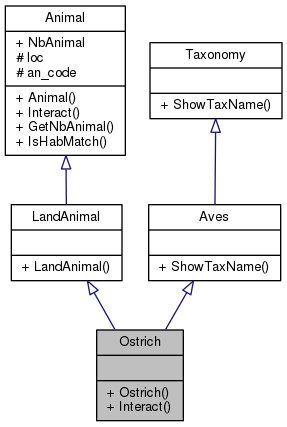
\includegraphics[width=284pt]{classOstrich__inherit__graph}
\end{center}
\end{figure}


Collaboration diagram for Ostrich\+:
\nopagebreak
\begin{figure}[H]
\begin{center}
\leavevmode
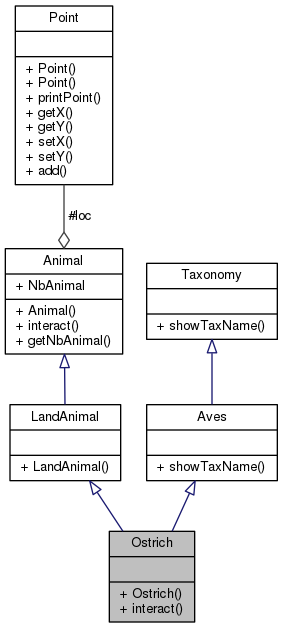
\includegraphics[width=284pt]{classOstrich__coll__graph}
\end{center}
\end{figure}
\subsection*{Public Member Functions}
\begin{DoxyCompactItemize}
\item 
\hyperlink{classOstrich_aba1eba1845346f98ace122c53d42754e}{Ostrich} (int x, int y)
\begin{DoxyCompactList}\small\item\em Constructor. \end{DoxyCompactList}\item 
void \hyperlink{classOstrich_a1bade94b6252e9d59bb82bf55ca1b29b}{interact} ()\hypertarget{classOstrich_a1bade94b6252e9d59bb82bf55ca1b29b}{}\label{classOstrich_a1bade94b6252e9d59bb82bf55ca1b29b}

\begin{DoxyCompactList}\small\item\em Method interaksi ostrich. \end{DoxyCompactList}\end{DoxyCompactItemize}
\subsection*{Additional Inherited Members}


\subsection{Detailed Description}
Real class ostrich 

\subsection{Constructor \& Destructor Documentation}
\index{Ostrich@{Ostrich}!Ostrich@{Ostrich}}
\index{Ostrich@{Ostrich}!Ostrich@{Ostrich}}
\subsubsection[{\texorpdfstring{Ostrich(int x, int y)}{Ostrich(int x, int y)}}]{\setlength{\rightskip}{0pt plus 5cm}Ostrich\+::\+Ostrich (
\begin{DoxyParamCaption}
\item[{int}]{x, }
\item[{int}]{y}
\end{DoxyParamCaption}
)}\hypertarget{classOstrich_aba1eba1845346f98ace122c53d42754e}{}\label{classOstrich_aba1eba1845346f98ace122c53d42754e}


Constructor. 


\begin{DoxyParams}{Parameters}
{\em x} & absis lokasi \\
\hline
{\em y} & ordinat lokasi Konstruktor kelas ostrich \\
\hline
\end{DoxyParams}


The documentation for this class was generated from the following files\+:\begin{DoxyCompactItemize}
\item 
Land\+Animal.\+h\item 
Land\+Animal.\+cpp\end{DoxyCompactItemize}

\hypertarget{classPanda}{}\section{Panda Class Reference}
\label{classPanda}\index{Panda@{Panda}}


{\ttfamily \#include $<$Land\+Animal.\+h$>$}



Inheritance diagram for Panda\+:
\nopagebreak
\begin{figure}[H]
\begin{center}
\leavevmode
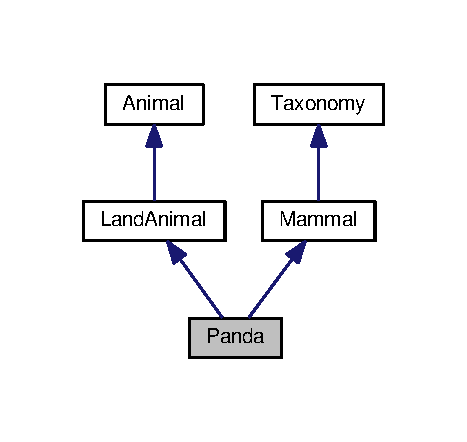
\includegraphics[width=284pt]{classPanda__inherit__graph}
\end{center}
\end{figure}


Collaboration diagram for Panda\+:
\nopagebreak
\begin{figure}[H]
\begin{center}
\leavevmode
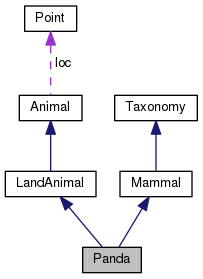
\includegraphics[width=284pt]{classPanda__coll__graph}
\end{center}
\end{figure}
\subsection*{Public Member Functions}
\begin{DoxyCompactItemize}
\item 
\hyperlink{classPanda_a9d007730c0a0dae0836e7be527610c42}{Panda} (int x, int y)
\begin{DoxyCompactList}\small\item\em Constructor. \end{DoxyCompactList}\item 
void \hyperlink{classPanda_a04e6a6078ef1240c1407fe1fd6c28237}{interact} ()\hypertarget{classPanda_a04e6a6078ef1240c1407fe1fd6c28237}{}\label{classPanda_a04e6a6078ef1240c1407fe1fd6c28237}

\begin{DoxyCompactList}\small\item\em Method interaksi panda. \end{DoxyCompactList}\end{DoxyCompactItemize}
\subsection*{Additional Inherited Members}


\subsection{Detailed Description}
Real class panda 

\subsection{Constructor \& Destructor Documentation}
\index{Panda@{Panda}!Panda@{Panda}}
\index{Panda@{Panda}!Panda@{Panda}}
\subsubsection[{\texorpdfstring{Panda(int x, int y)}{Panda(int x, int y)}}]{\setlength{\rightskip}{0pt plus 5cm}Panda\+::\+Panda (
\begin{DoxyParamCaption}
\item[{int}]{x, }
\item[{int}]{y}
\end{DoxyParamCaption}
)}\hypertarget{classPanda_a9d007730c0a0dae0836e7be527610c42}{}\label{classPanda_a9d007730c0a0dae0836e7be527610c42}


Constructor. 


\begin{DoxyParams}{Parameters}
{\em x} & absis lokasi \\
\hline
{\em y} & ordinat lokasi Konstruktor kelas panda \\
\hline
\end{DoxyParams}


The documentation for this class was generated from the following files\+:\begin{DoxyCompactItemize}
\item 
Land\+Animal.\+h\item 
Land\+Animal.\+cpp\end{DoxyCompactItemize}

\hypertarget{classPark}{}\section{Park Class Reference}
\label{classPark}\index{Park@{Park}}


{\ttfamily \#include $<$Facility.\+h$>$}



Inheritance diagram for Park\+:
\nopagebreak
\begin{figure}[H]
\begin{center}
\leavevmode
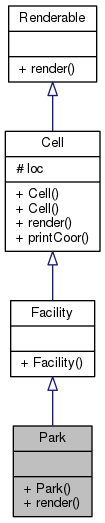
\includegraphics[width=146pt]{classPark__inherit__graph}
\end{center}
\end{figure}


Collaboration diagram for Park\+:
\nopagebreak
\begin{figure}[H]
\begin{center}
\leavevmode
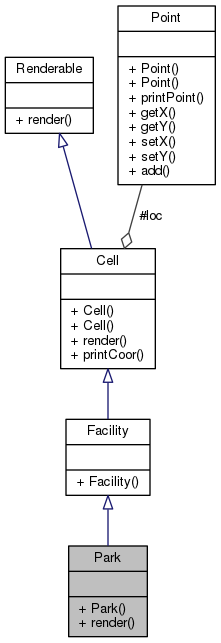
\includegraphics[width=204pt]{classPark__coll__graph}
\end{center}
\end{figure}
\subsection*{Public Member Functions}
\begin{DoxyCompactItemize}
\item 
\hyperlink{classPark_a2d682e911b7209d46ddabbf3d7cd2165}{Park} (int x, int y)
\begin{DoxyCompactList}\small\item\em Constructor. \end{DoxyCompactList}\item 
void \hyperlink{classPark_afd7fe6ec511aab1b2451096b54c3addd}{render} ()\hypertarget{classPark_afd7fe6ec511aab1b2451096b54c3addd}{}\label{classPark_afd7fe6ec511aab1b2451096b54c3addd}

\begin{DoxyCompactList}\small\item\em Method render. \end{DoxyCompactList}\end{DoxyCompactItemize}
\subsection*{Additional Inherited Members}


\subsection{Detailed Description}
Real class park 

\subsection{Constructor \& Destructor Documentation}
\index{Park@{Park}!Park@{Park}}
\index{Park@{Park}!Park@{Park}}
\subsubsection[{\texorpdfstring{Park(int x, int y)}{Park(int x, int y)}}]{\setlength{\rightskip}{0pt plus 5cm}Park\+::\+Park (
\begin{DoxyParamCaption}
\item[{int}]{x, }
\item[{int}]{y}
\end{DoxyParamCaption}
)}\hypertarget{classPark_a2d682e911b7209d46ddabbf3d7cd2165}{}\label{classPark_a2d682e911b7209d46ddabbf3d7cd2165}


Constructor. 


\begin{DoxyParams}{Parameters}
{\em x} & absis lokasi \\
\hline
{\em y} & oridnat lokasi Konstruktor kelas park \\
\hline
\end{DoxyParams}


The documentation for this class was generated from the following files\+:\begin{DoxyCompactItemize}
\item 
Facility.\+h\item 
Facility.\+cpp\end{DoxyCompactItemize}

\hypertarget{classPeacock}{}\section{Peacock Class Reference}
\label{classPeacock}\index{Peacock@{Peacock}}


{\ttfamily \#include $<$Land\+Animal.\+h$>$}



Inheritance diagram for Peacock\+:
% FIG 0


Collaboration diagram for Peacock\+:
% FIG 1
\subsection*{Public Member Functions}
\begin{DoxyCompactItemize}
\item 
\hyperlink{classPeacock_a1a0c18540a84e95bf3dfa4f74a62ef79}{Peacock} (int x, int y)
\begin{DoxyCompactList}\small\item\em Constructor. \end{DoxyCompactList}\item 
void \hyperlink{classPeacock_abe13b72bf7b86c0e1168a9253f68015e}{interact} ()\hypertarget{classPeacock_abe13b72bf7b86c0e1168a9253f68015e}{}\label{classPeacock_abe13b72bf7b86c0e1168a9253f68015e}

\begin{DoxyCompactList}\small\item\em Method interaksi peacock. \end{DoxyCompactList}\end{DoxyCompactItemize}
\subsection*{Additional Inherited Members}


\subsection{Detailed Description}
Real class peacock 

\subsection{Constructor \& Destructor Documentation}
\index{Peacock@{Peacock}!Peacock@{Peacock}}
\index{Peacock@{Peacock}!Peacock@{Peacock}}
\subsubsection[{\texorpdfstring{Peacock(int x, int y)}{Peacock(int x, int y)}}]{\setlength{\rightskip}{0pt plus 5cm}Peacock\+::\+Peacock (
\begin{DoxyParamCaption}
\item[{int}]{x, }
\item[{int}]{y}
\end{DoxyParamCaption}
)}\hypertarget{classPeacock_a1a0c18540a84e95bf3dfa4f74a62ef79}{}\label{classPeacock_a1a0c18540a84e95bf3dfa4f74a62ef79}


Constructor. 


\begin{DoxyParams}{Parameters}
{\em x} & absis lokasi \\
\hline
{\em y} & ordinat lokasi Konstruktor kelas peacock \\
\hline
\end{DoxyParams}


The documentation for this class was generated from the following files\+:\begin{DoxyCompactItemize}
\item 
Land\+Animal.\+h\item 
Land\+Animal.\+cpp\end{DoxyCompactItemize}

\hypertarget{classPisces}{}\section{Pisces Class Reference}
\label{classPisces}\index{Pisces@{Pisces}}


{\ttfamily \#include $<$pisces.\+h$>$}



Inheritance diagram for Pisces\+:
% FIG 0


Collaboration diagram for Pisces\+:
% FIG 1
\subsection*{Public Member Functions}
\begin{DoxyCompactItemize}
\item 
void \hyperlink{classPisces_ab12b83c0263c81c275f1372b4038c023}{Show\+Tax\+Name} ()\hypertarget{classPisces_ab12b83c0263c81c275f1372b4038c023}{}\label{classPisces_ab12b83c0263c81c275f1372b4038c023}

\begin{DoxyCompactList}\small\item\em method Show\+Name. Menampilkan nama taksonomi. \end{DoxyCompactList}\end{DoxyCompactItemize}


\subsection{Detailed Description}
Base class 

The documentation for this class was generated from the following files\+:\begin{DoxyCompactItemize}
\item 
pisces/pisces.\+h\item 
pisces/pisces.\+cpp\end{DoxyCompactItemize}

\hypertarget{classPoint}{}\section{Point Class Reference}
\label{classPoint}\index{Point@{Point}}


Collaboration diagram for Point\+:
\nopagebreak
\begin{figure}[H]
\begin{center}
\leavevmode
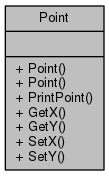
\includegraphics[width=153pt]{classPoint__coll__graph}
\end{center}
\end{figure}
\subsection*{Public Member Functions}
\begin{DoxyCompactItemize}
\item 
{\bfseries Point} (int x, int y)\hypertarget{classPoint_a001c4958c310b248f5c26037aea38a9c}{}\label{classPoint_a001c4958c310b248f5c26037aea38a9c}

\item 
{\bfseries Point} (const \hyperlink{classPoint}{Point} \&P)\hypertarget{classPoint_a7e32c5a7f878c49ed9f1777b622cc06c}{}\label{classPoint_a7e32c5a7f878c49ed9f1777b622cc06c}

\item 
void {\bfseries print\+Point} ()\hypertarget{classPoint_ad32f6a515be1cf069bf5ea6b89178ae9}{}\label{classPoint_ad32f6a515be1cf069bf5ea6b89178ae9}

\item 
int {\bfseries getX} () const \hypertarget{classPoint_abe622fffc8785b0c2e06cdac681b9837}{}\label{classPoint_abe622fffc8785b0c2e06cdac681b9837}

\item 
int {\bfseries getY} () const \hypertarget{classPoint_a10f31e48e2dbc22e3660ca769b8d5d65}{}\label{classPoint_a10f31e48e2dbc22e3660ca769b8d5d65}

\item 
void {\bfseries setX} (int x)\hypertarget{classPoint_acdc86ab607b2ae8415152883e2629015}{}\label{classPoint_acdc86ab607b2ae8415152883e2629015}

\item 
void {\bfseries setY} (int y)\hypertarget{classPoint_afccad787a359f062efc1af5e935a99ba}{}\label{classPoint_afccad787a359f062efc1af5e935a99ba}

\item 
void {\bfseries add} (int x, int y)\hypertarget{classPoint_a339fe8d180ebbc9079d349c23dc477fe}{}\label{classPoint_a339fe8d180ebbc9079d349c23dc477fe}

\end{DoxyCompactItemize}


The documentation for this class was generated from the following files\+:\begin{DoxyCompactItemize}
\item 
Point.\+h\item 
Point.\+cpp\end{DoxyCompactItemize}

\hypertarget{classRenderable}{}\section{Renderable Class Reference}
\label{classRenderable}\index{Renderable@{Renderable}}


Inheritance diagram for Renderable\+:
\nopagebreak
\begin{figure}[H]
\begin{center}
\leavevmode
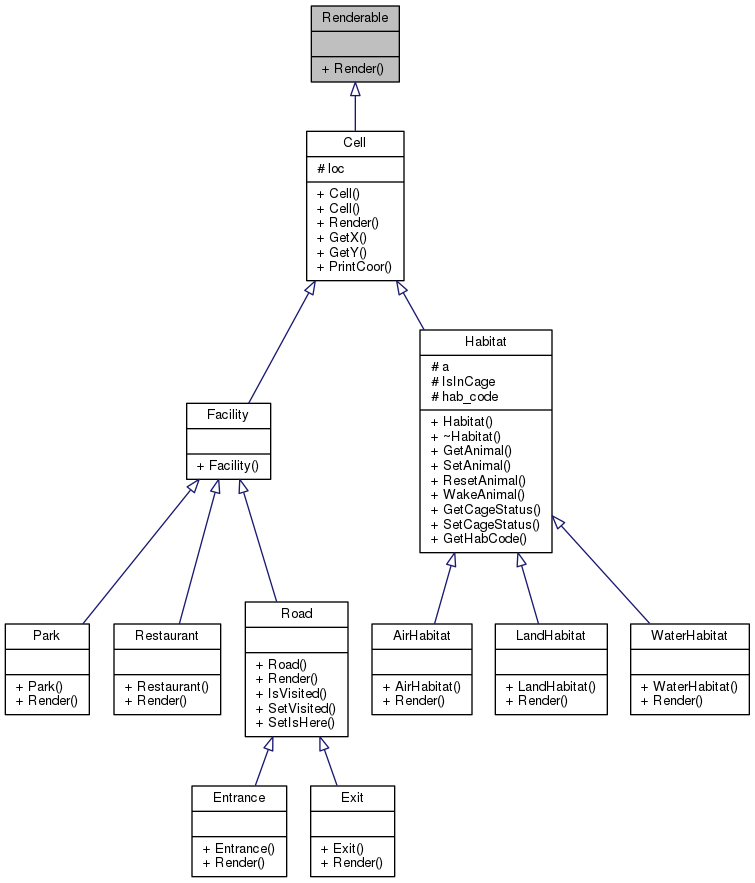
\includegraphics[width=350pt]{classRenderable__inherit__graph}
\end{center}
\end{figure}
\subsection*{Public Member Functions}
\begin{DoxyCompactItemize}
\item 
virtual void {\bfseries render} ()=0\hypertarget{classRenderable_a7d02709d871bd2bde97d41d933df5adf}{}\label{classRenderable_a7d02709d871bd2bde97d41d933df5adf}

\end{DoxyCompactItemize}


The documentation for this class was generated from the following file\+:\begin{DoxyCompactItemize}
\item 
Renderable.\+h\end{DoxyCompactItemize}

\hypertarget{classReptile}{}\section{Reptile Class Reference}
\label{classReptile}\index{Reptile@{Reptile}}


{\ttfamily \#include $<$reptile.\+h$>$}



Inheritance diagram for Reptile\+:
% FIG 0


Collaboration diagram for Reptile\+:
% FIG 1
\subsection*{Public Member Functions}
\begin{DoxyCompactItemize}
\item 
void \hyperlink{classReptile_a4ca008392f1818081052313071d87a8a}{Show\+Tax\+Name} ()\hypertarget{classReptile_a4ca008392f1818081052313071d87a8a}{}\label{classReptile_a4ca008392f1818081052313071d87a8a}

\begin{DoxyCompactList}\small\item\em method Show\+Name. Menampilkan nama taksonomi. \end{DoxyCompactList}\end{DoxyCompactItemize}


\subsection{Detailed Description}
Base class 

The documentation for this class was generated from the following files\+:\begin{DoxyCompactItemize}
\item 
reptile/reptile.\+h\item 
reptile/reptile.\+cpp\end{DoxyCompactItemize}

\hypertarget{classRestaurant}{}\section{Restaurant Class Reference}
\label{classRestaurant}\index{Restaurant@{Restaurant}}


{\ttfamily \#include $<$Facility.\+h$>$}



Inheritance diagram for Restaurant\+:
% FIG 0


Collaboration diagram for Restaurant\+:
% FIG 1
\subsection*{Public Member Functions}
\begin{DoxyCompactItemize}
\item 
\hyperlink{classRestaurant_a95f0844bcee4b2bc717d0c2bd70bb496}{Restaurant} (int x, int y)
\begin{DoxyCompactList}\small\item\em Constructor. \end{DoxyCompactList}\item 
void \hyperlink{classRestaurant_a922ef15598aa096dcfe9b9903d181180}{render} ()\hypertarget{classRestaurant_a922ef15598aa096dcfe9b9903d181180}{}\label{classRestaurant_a922ef15598aa096dcfe9b9903d181180}

\begin{DoxyCompactList}\small\item\em Method render. \end{DoxyCompactList}\end{DoxyCompactItemize}
\subsection*{Additional Inherited Members}


\subsection{Detailed Description}
Real class restaurant 

\subsection{Constructor \& Destructor Documentation}
\index{Restaurant@{Restaurant}!Restaurant@{Restaurant}}
\index{Restaurant@{Restaurant}!Restaurant@{Restaurant}}
\subsubsection[{\texorpdfstring{Restaurant(int x, int y)}{Restaurant(int x, int y)}}]{\setlength{\rightskip}{0pt plus 5cm}Restaurant\+::\+Restaurant (
\begin{DoxyParamCaption}
\item[{int}]{x, }
\item[{int}]{y}
\end{DoxyParamCaption}
)}\hypertarget{classRestaurant_a95f0844bcee4b2bc717d0c2bd70bb496}{}\label{classRestaurant_a95f0844bcee4b2bc717d0c2bd70bb496}


Constructor. 


\begin{DoxyParams}{Parameters}
{\em x} & absis lokasi \\
\hline
{\em y} & oridnat lokasi Konstruktor kelas restaurant \\
\hline
\end{DoxyParams}


The documentation for this class was generated from the following files\+:\begin{DoxyCompactItemize}
\item 
Facility.\+h\item 
Facility.\+cpp\end{DoxyCompactItemize}

\hypertarget{classRoad}{}\section{Road Class Reference}
\label{classRoad}\index{Road@{Road}}


{\ttfamily \#include $<$road.\+h$>$}



Inheritance diagram for Road\+:
% FIG 0


Collaboration diagram for Road\+:
% FIG 1
\subsection*{Public Member Functions}
\begin{DoxyCompactItemize}
\item 
\hyperlink{classRoad_adf96d914718db461bddfbc5e5a0312cc}{Road} (int x, int y)
\begin{DoxyCompactList}\small\item\em Constructor. \end{DoxyCompactList}\item 
virtual void \hyperlink{classRoad_a1a765835fb4bd7c64d12a511a72552b9}{Render} ()\hypertarget{classRoad_a1a765835fb4bd7c64d12a511a72552b9}{}\label{classRoad_a1a765835fb4bd7c64d12a511a72552b9}

\begin{DoxyCompactList}\small\item\em Method virtual render. \end{DoxyCompactList}\item 
bool {\bfseries Is\+Visited} ()\hypertarget{classRoad_a2015eb6ca5c6a3b9f3d2e4fd13eb8e05}{}\label{classRoad_a2015eb6ca5c6a3b9f3d2e4fd13eb8e05}

\item 
void {\bfseries Set\+Visited} (bool s)\hypertarget{classRoad_a12f23535261fa769f0f26b8b450c1e9f}{}\label{classRoad_a12f23535261fa769f0f26b8b450c1e9f}

\item 
void {\bfseries Set\+Is\+Here} (bool s)\hypertarget{classRoad_a86de16ad0c78e6638a5803572b71bdf5}{}\label{classRoad_a86de16ad0c78e6638a5803572b71bdf5}

\end{DoxyCompactItemize}
\subsection*{Additional Inherited Members}


\subsection{Detailed Description}
Real class road 

\subsection{Constructor \& Destructor Documentation}
\index{Road@{Road}!Road@{Road}}
\index{Road@{Road}!Road@{Road}}
\subsubsection[{\texorpdfstring{Road(int x, int y)}{Road(int x, int y)}}]{\setlength{\rightskip}{0pt plus 5cm}Road\+::\+Road (
\begin{DoxyParamCaption}
\item[{int}]{x, }
\item[{int}]{y}
\end{DoxyParamCaption}
)}\hypertarget{classRoad_adf96d914718db461bddfbc5e5a0312cc}{}\label{classRoad_adf96d914718db461bddfbc5e5a0312cc}


Constructor. 


\begin{DoxyParams}{Parameters}
{\em x} & absis lokasi \\
\hline
{\em y} & oridnat lokasi Konstruktor kelas road \\
\hline
\end{DoxyParams}


The documentation for this class was generated from the following files\+:\begin{DoxyCompactItemize}
\item 
road/road.\+h\item 
road/road.\+cpp\end{DoxyCompactItemize}

\hypertarget{classShark}{}\section{Shark Class Reference}
\label{classShark}\index{Shark@{Shark}}


{\ttfamily \#include $<$Water\+Animal.\+h$>$}



Inheritance diagram for Shark\+:
\nopagebreak
\begin{figure}[H]
\begin{center}
\leavevmode
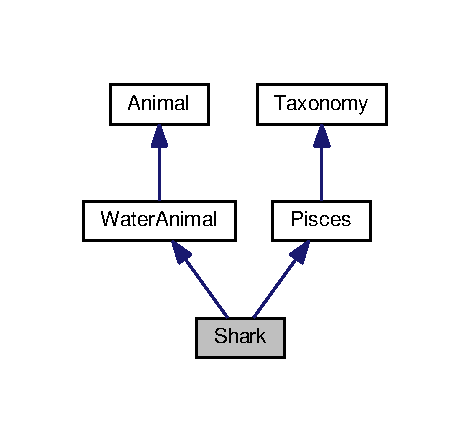
\includegraphics[width=226pt]{classShark__inherit__graph}
\end{center}
\end{figure}


Collaboration diagram for Shark\+:
\nopagebreak
\begin{figure}[H]
\begin{center}
\leavevmode
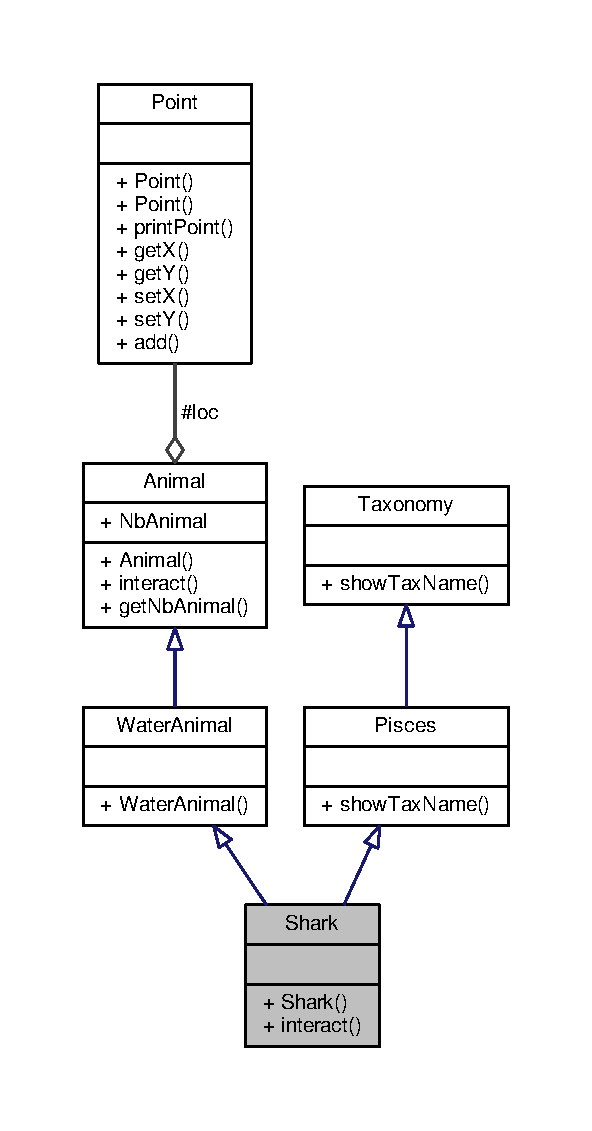
\includegraphics[width=226pt]{classShark__coll__graph}
\end{center}
\end{figure}
\subsection*{Public Member Functions}
\begin{DoxyCompactItemize}
\item 
\hyperlink{classShark_a4ea94f8c6678e7275bb84820b2944f4c}{Shark} (int x, int y)
\begin{DoxyCompactList}\small\item\em Constructor. \end{DoxyCompactList}\item 
void \hyperlink{classShark_ad643ad27db3da8fad65890bba6a1b252}{interact} ()\hypertarget{classShark_ad643ad27db3da8fad65890bba6a1b252}{}\label{classShark_ad643ad27db3da8fad65890bba6a1b252}

\begin{DoxyCompactList}\small\item\em Method interaksi shark. \end{DoxyCompactList}\end{DoxyCompactItemize}
\subsection*{Additional Inherited Members}


\subsection{Detailed Description}
Real class shark 

\subsection{Constructor \& Destructor Documentation}
\index{Shark@{Shark}!Shark@{Shark}}
\index{Shark@{Shark}!Shark@{Shark}}
\subsubsection[{\texorpdfstring{Shark(int x, int y)}{Shark(int x, int y)}}]{\setlength{\rightskip}{0pt plus 5cm}Shark\+::\+Shark (
\begin{DoxyParamCaption}
\item[{int}]{x, }
\item[{int}]{y}
\end{DoxyParamCaption}
)}\hypertarget{classShark_a4ea94f8c6678e7275bb84820b2944f4c}{}\label{classShark_a4ea94f8c6678e7275bb84820b2944f4c}


Constructor. 


\begin{DoxyParams}{Parameters}
{\em x} & absis lokasi \\
\hline
{\em y} & ordinat lokasi Konstruktor kelas shark \\
\hline
\end{DoxyParams}


The documentation for this class was generated from the following files\+:\begin{DoxyCompactItemize}
\item 
Water\+Animal.\+h\item 
Water\+Animal.\+cpp\end{DoxyCompactItemize}

\hypertarget{classTaxonomy}{}\section{Taxonomy Class Reference}
\label{classTaxonomy}\index{Taxonomy@{Taxonomy}}


Inheritance diagram for Taxonomy\+:
\nopagebreak
\begin{figure}[H]
\begin{center}
\leavevmode
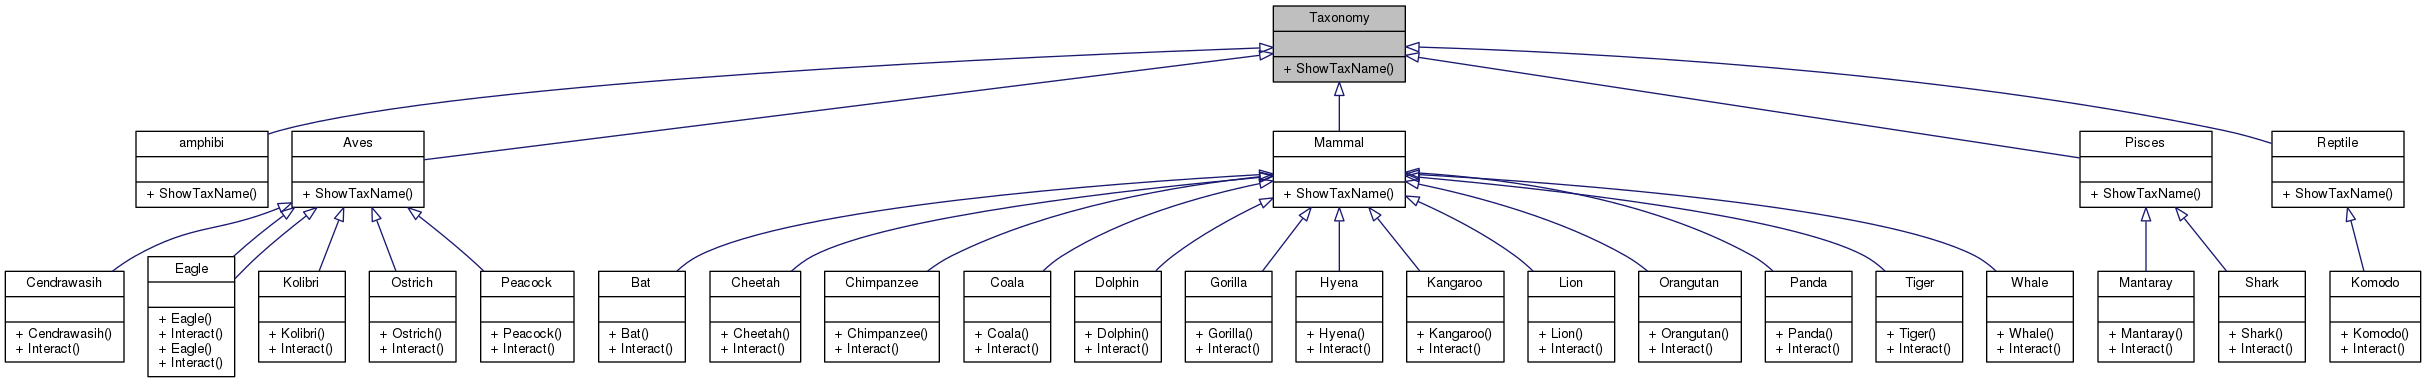
\includegraphics[width=350pt]{classTaxonomy__inherit__graph}
\end{center}
\end{figure}


Collaboration diagram for Taxonomy\+:
\nopagebreak
\begin{figure}[H]
\begin{center}
\leavevmode
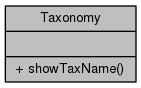
\includegraphics[width=178pt]{classTaxonomy__coll__graph}
\end{center}
\end{figure}
\subsection*{Public Member Functions}
\begin{DoxyCompactItemize}
\item 
virtual void {\bfseries show\+Tax\+Name} ()=0\hypertarget{classTaxonomy_aedc7597a50cc7fd4d6bdcbe370e8a414}{}\label{classTaxonomy_aedc7597a50cc7fd4d6bdcbe370e8a414}

\end{DoxyCompactItemize}


The documentation for this class was generated from the following file\+:\begin{DoxyCompactItemize}
\item 
Taxonomy.\+h\end{DoxyCompactItemize}

\hypertarget{classTiger}{}\section{Tiger Class Reference}
\label{classTiger}\index{Tiger@{Tiger}}


{\ttfamily \#include $<$tiger.\+h$>$}



Inheritance diagram for Tiger\+:
% FIG 0


Collaboration diagram for Tiger\+:
% FIG 1
\subsection*{Public Member Functions}
\begin{DoxyCompactItemize}
\item 
\hyperlink{classTiger_aa4604524d55c97444310b333228ad456}{Tiger} (int x, int y, int \hyperlink{classAnimal_a9a3b22f243f7109c57f36b3c660feb6e}{weight})
\begin{DoxyCompactList}\small\item\em Constructor. \end{DoxyCompactList}\item 
void \hyperlink{classTiger_ac9661764d305a083a94522023e9aa311}{Render\+Animal} ()\hypertarget{classTiger_ac9661764d305a083a94522023e9aa311}{}\label{classTiger_ac9661764d305a083a94522023e9aa311}

\begin{DoxyCompactList}\small\item\em Method interaksi tiger. \end{DoxyCompactList}\item 
void {\bfseries Interact} ()\hypertarget{classTiger_a7ab54d45a36306f9c4fd3af6fb5f5118}{}\label{classTiger_a7ab54d45a36306f9c4fd3af6fb5f5118}

\end{DoxyCompactItemize}
\subsection*{Additional Inherited Members}


\subsection{Detailed Description}
Real class tiger 

\subsection{Constructor \& Destructor Documentation}
\index{Tiger@{Tiger}!Tiger@{Tiger}}
\index{Tiger@{Tiger}!Tiger@{Tiger}}
\subsubsection[{\texorpdfstring{Tiger(int x, int y, int weight)}{Tiger(int x, int y, int weight)}}]{\setlength{\rightskip}{0pt plus 5cm}Tiger\+::\+Tiger (
\begin{DoxyParamCaption}
\item[{int}]{x, }
\item[{int}]{y, }
\item[{int}]{weight}
\end{DoxyParamCaption}
)}\hypertarget{classTiger_aa4604524d55c97444310b333228ad456}{}\label{classTiger_aa4604524d55c97444310b333228ad456}


Constructor. 


\begin{DoxyParams}{Parameters}
{\em x} & absis lokasi \\
\hline
{\em y} & ordinat lokasi \\
\hline
{\em weight} & berat badan Konstruktor kelas tiger \\
\hline
\end{DoxyParams}


The documentation for this class was generated from the following files\+:\begin{DoxyCompactItemize}
\item 
tiger/tiger.\+h\item 
tiger/tiger.\+cpp\end{DoxyCompactItemize}

\hypertarget{classWaterAnimal}{}\section{Water\+Animal Class Reference}
\label{classWaterAnimal}\index{Water\+Animal@{Water\+Animal}}


Inheritance diagram for Water\+Animal\+:
% FIG 0


Collaboration diagram for Water\+Animal\+:
% FIG 1
\subsection*{Public Member Functions}
\begin{DoxyCompactItemize}
\item 
{\bfseries Water\+Animal} (int x, int y)\hypertarget{classWaterAnimal_ab11245c8547382631a6ae1053443ad72}{}\label{classWaterAnimal_ab11245c8547382631a6ae1053443ad72}

\end{DoxyCompactItemize}
\subsection*{Additional Inherited Members}


The documentation for this class was generated from the following files\+:\begin{DoxyCompactItemize}
\item 
Animal.\+h\item 
Animal.\+cpp\end{DoxyCompactItemize}

\hypertarget{classWaterHabitat}{}\section{Water\+Habitat Class Reference}
\label{classWaterHabitat}\index{Water\+Habitat@{Water\+Habitat}}


{\ttfamily \#include $<$water\+\_\+habitat.\+h$>$}



Inheritance diagram for Water\+Habitat\+:
% FIG 0


Collaboration diagram for Water\+Habitat\+:
% FIG 1
\subsection*{Public Member Functions}
\begin{DoxyCompactItemize}
\item 
\hyperlink{classWaterHabitat_af86ce59bbb950ef716cad385eacd5227}{Water\+Habitat} (int x, int y, bool s)
\begin{DoxyCompactList}\small\item\em \hyperlink{classWaterHabitat}{Water\+Habitat}. \end{DoxyCompactList}\item 
void \hyperlink{classWaterHabitat_abcd9e7dff3c25b78665979ef47fb4a7d}{Render} ()\hypertarget{classWaterHabitat_abcd9e7dff3c25b78665979ef47fb4a7d}{}\label{classWaterHabitat_abcd9e7dff3c25b78665979ef47fb4a7d}

\begin{DoxyCompactList}\small\item\em Method render. \end{DoxyCompactList}\end{DoxyCompactItemize}
\subsection*{Additional Inherited Members}


\subsection{Detailed Description}
Base class waterhabitat 

\subsection{Constructor \& Destructor Documentation}
\index{Water\+Habitat@{Water\+Habitat}!Water\+Habitat@{Water\+Habitat}}
\index{Water\+Habitat@{Water\+Habitat}!Water\+Habitat@{Water\+Habitat}}
\subsubsection[{\texorpdfstring{Water\+Habitat(int x, int y, bool s)}{WaterHabitat(int x, int y, bool s)}}]{\setlength{\rightskip}{0pt plus 5cm}Water\+Habitat\+::\+Water\+Habitat (
\begin{DoxyParamCaption}
\item[{int}]{x, }
\item[{int}]{y, }
\item[{bool}]{s}
\end{DoxyParamCaption}
)}\hypertarget{classWaterHabitat_af86ce59bbb950ef716cad385eacd5227}{}\label{classWaterHabitat_af86ce59bbb950ef716cad385eacd5227}


\hyperlink{classWaterHabitat}{Water\+Habitat}. 


\begin{DoxyParams}{Parameters}
{\em x} & absis lokasi \\
\hline
{\em y} & oridnat lokasi Konstruktor waterhabitat \\
\hline
\end{DoxyParams}


The documentation for this class was generated from the following files\+:\begin{DoxyCompactItemize}
\item 
water\+\_\+habitat/water\+\_\+habitat.\+h\item 
water\+\_\+habitat/water\+\_\+habitat.\+cpp\end{DoxyCompactItemize}

\hypertarget{classWhale}{}\section{Whale Class Reference}
\label{classWhale}\index{Whale@{Whale}}


{\ttfamily \#include $<$whale.\+h$>$}



Inheritance diagram for Whale\+:
% FIG 0


Collaboration diagram for Whale\+:
% FIG 1
\subsection*{Public Member Functions}
\begin{DoxyCompactItemize}
\item 
\hyperlink{classWhale_a00d149a599c0d568f20ca885c00d80d2}{Whale} (int x, int y, int \hyperlink{classAnimal_a9a3b22f243f7109c57f36b3c660feb6e}{weight})
\begin{DoxyCompactList}\small\item\em Constructor. \end{DoxyCompactList}\item 
void \hyperlink{classWhale_adac10dde379734b0c71fce7aa5a27be4}{Interact} ()\hypertarget{classWhale_adac10dde379734b0c71fce7aa5a27be4}{}\label{classWhale_adac10dde379734b0c71fce7aa5a27be4}

\begin{DoxyCompactList}\small\item\em Method interaksi whale. \end{DoxyCompactList}\item 
void {\bfseries Render\+Animal} ()\hypertarget{classWhale_a64773ba49e5ab23521e28e076e8ecb93}{}\label{classWhale_a64773ba49e5ab23521e28e076e8ecb93}

\end{DoxyCompactItemize}
\subsection*{Additional Inherited Members}


\subsection{Detailed Description}
Real class whale 

\subsection{Constructor \& Destructor Documentation}
\index{Whale@{Whale}!Whale@{Whale}}
\index{Whale@{Whale}!Whale@{Whale}}
\subsubsection[{\texorpdfstring{Whale(int x, int y, int weight)}{Whale(int x, int y, int weight)}}]{\setlength{\rightskip}{0pt plus 5cm}Whale\+::\+Whale (
\begin{DoxyParamCaption}
\item[{int}]{x, }
\item[{int}]{y, }
\item[{int}]{weight}
\end{DoxyParamCaption}
)}\hypertarget{classWhale_a00d149a599c0d568f20ca885c00d80d2}{}\label{classWhale_a00d149a599c0d568f20ca885c00d80d2}


Constructor. 


\begin{DoxyParams}{Parameters}
{\em x} & absis lokasi \\
\hline
{\em y} & ordinat lokasi \\
\hline
{\em weight} & berat badan Konstruktor kelas whale \\
\hline
\end{DoxyParams}


The documentation for this class was generated from the following files\+:\begin{DoxyCompactItemize}
\item 
whale/whale.\+h\item 
whale/whale.\+cpp\end{DoxyCompactItemize}

\hypertarget{classZoo}{}\section{Zoo Class Reference}
\label{classZoo}\index{Zoo@{Zoo}}
\subsection*{Public Member Functions}
\begin{DoxyCompactItemize}
\item 
{\bfseries Zoo} (int w, int h)\hypertarget{classZoo_a5e4518eccc8e44d23c4b0f37e7e503cc}{}\label{classZoo_a5e4518eccc8e44d23c4b0f37e7e503cc}

\item 
void {\bfseries initialize} (char $\ast$$\ast$c, int row, int col)\hypertarget{classZoo_a8236fa2a39cd2c6c4535d638d2edee1c}{}\label{classZoo_a8236fa2a39cd2c6c4535d638d2edee1c}

\item 
void {\bfseries show} ()\hypertarget{classZoo_aed92b968c2bb9dd83993cc7707b1b6b9}{}\label{classZoo_aed92b968c2bb9dd83993cc7707b1b6b9}

\end{DoxyCompactItemize}


The documentation for this class was generated from the following files\+:\begin{DoxyCompactItemize}
\item 
Zoo.\+h\item 
Zoo.\+cpp\end{DoxyCompactItemize}

%--- End generated contents ---

% Index
\backmatter
\newpage
\phantomsection
\clearemptydoublepage
\addcontentsline{toc}{chapter}{Index}
\printindex

\end{document}
